% !TEX program = pdflatex
% CSC263 - Combined Lecture Notes (Lectures 1 & 2)
% Organized notes for TeXShop
\documentclass[11pt]{article}

\usepackage[utf8]{inputenc}
\usepackage[T1]{fontenc}
\usepackage[a4paper,margin=2.4cm]{geometry}
\usepackage{amsmath,amssymb,amsthm,mathtools}
\usepackage{xcolor}
\usepackage[most]{tcolorbox}
\usepackage{tikz}
\usepackage{pgfplots}
\pgfplotsset{compat=1.17}
\usetikzlibrary{arrows.meta,calc,backgrounds,decorations.pathmorphing}
\usepackage{enumitem}
\usepackage[protrusion=true,expansion=false]{microtype}
\usepackage[colorlinks=true,linkcolor=violetT,urlcolor=violetT]{hyperref}
\usepackage{fancyhdr}
\usepackage{sectsty}

% ------------------------------------------------------------------
%  COLOURS
% ------------------------------------------------------------------
\definecolor{violetT}{HTML}{5B4F9E}
\definecolor{greenO}{HTML}{4E9A3D}   % O, "every", "at most", upper bound
\definecolor{rustW}{HTML}{B0561F}    % Omega, "some", "at least", lower bound
\definecolor{heapblue}{HTML}{2F6DB5} % tree nodes / edges
\definecolor{skyfill}{HTML}{E8F3FA}
\definecolor{defblue}{HTML}{2F6DB5}
\definecolor{deffill}{HTML}{EAF1FB}
\definecolor{greyline}{HTML}{9AA0A6}
\definecolor{amber}{HTML}{C7891F}
\definecolor{amberfill}{HTML}{FBF3E0}
\definecolor{utnavy}{HTML}{102A54}
\definecolor{goldpath}{HTML}{E8A32C}
\definecolor{inkT}{HTML}{3A3A3A}

% semantic shortcuts
\newcommand{\Obig}{\textcolor{greenO}{$O$}}
\newcommand{\Wbig}{\textcolor{rustW}{$\Omega$}}
\newcommand{\Tbig}{\textcolor{violetT}{$\Theta$}}
\newcommand{\every}{\textcolor{greenO}{\textbf{every}}}
\newcommand{\atmost}{\textcolor{greenO}{\textbf{at most}}}
\newcommand{\some}{\textcolor{rustW}{\textbf{some}}}
\newcommand{\atleast}{\textcolor{rustW}{\textbf{at least}}}
\newcommand{\up}{\textcolor{greenO}{upper bound}}
\newcommand{\low}{\textcolor{rustW}{lower bound}}

% ------------------------------------------------------------------
%  BOXES
% ------------------------------------------------------------------
\newtcolorbox{defbox}[1][]{colback=deffill,colframe=defblue,coltitle=white,
  fonttitle=\bfseries,title={#1},boxrule=0.9pt,arc=3pt,left=6pt,right=6pt,top=5pt,bottom=5pt,breakable}

\newtcolorbox{keybox}[1][]{colback=skyfill,colframe=violetT,coltitle=white,
  fonttitle=\bfseries,title={#1},boxrule=0.9pt,arc=3pt,left=6pt,right=6pt,top=5pt,bottom=5pt,breakable}

\newtcolorbox{codebox}[1][]{colback=black!3,colframe=greyline,coltitle=black,
  fonttitle=\bfseries,title={#1},boxrule=0.6pt,arc=1pt,left=6pt,right=6pt,top=4pt,bottom=4pt,breakable}

\newtcolorbox{exambox}[1][Seen on a past exam]{enhanced,breakable,
  colback=amberfill,colframe=amber,coltitle=white,colbacktitle=amber,fonttitle=\bfseries,
  title={\raisebox{-1pt}{\large$\bigstar$}\; #1},boxrule=1.1pt,arc=3pt,left=7pt,right=7pt,top=6pt,bottom=6pt,drop shadow}

\newtcolorbox{answerband}{colback=white,colframe=greenO,boxrule=0.8pt,arc=2pt,left=6pt,right=6pt,top=4pt,bottom=4pt}

\newtcolorbox{warnbox}[1][]{enhanced,colback=amberfill,colframe=amber,coltitle=amber,
  fonttitle=\bfseries,title={#1},boxrule=0.8pt,arc=2pt,left=6pt,right=6pt,top=4pt,bottom=4pt,breakable}

\newtcolorbox{examplebox}[1][]{enhanced,colback=white,colframe=violetT!70,
  colbacktitle=violetT!10,coltitle=violetT,fonttitle=\bfseries,title={#1},
  boxrule=0.8pt,arc=2pt,left=6pt,right=6pt,top=4pt,bottom=4pt,breakable}

\allsectionsfont{\color{violetT}}
\setlength{\parindent}{0pt}
\setlength{\parskip}{5pt}

% ------------------------------------------------------------------
%  HEAP DRAWING MACROS
% ------------------------------------------------------------------
\tikzset{
  hnode/.style={circle,draw=heapblue,line width=0.7pt,minimum size=0.74cm,inner sep=0pt,font=\small\bfseries,fill=white},
  hedge/.style={heapblue,line width=0.7pt},
  hidx/.style={font=\scriptsize\bfseries,text=rustW}
}
\newcommand{\heapcoords}{\foreach \hi/\hx/\hy in {1/0/4.5,2/-2.3/3.0,3/2.3/3.0,4/-3.45/1.6,5/-1.15/1.6,6/1.15/1.6,7/3.45/1.6,8/-4.0/0.2,9/-2.9/0.2,10/-1.75/0.2}{\coordinate (p\hi) at (\hx,\hy);}}
\newcommand{\drawheap}[2]{%
  \heapcoords
  \begin{scope}[on background layer]\foreach \a/\b in {#2}{\draw[hedge] (p\a)--(p\b);}\end{scope}
  \foreach \idx/\val/\col in {#1}{%
     \node[hnode,text=\col] (n\idx) at (p\idx) {\val};
     \node[hidx] at ([shift={(-0.30,0.30)}]p\idx) {\idx};}
}
\newcommand{\heaparray}[1]{%
 \begin{tikzpicture}[scale=0.82]
 \node at (0.35,0.45) {\bfseries A:};
 \foreach \val [count=\i from 1] in {#1}{%
   \draw[line width=0.6pt] (\i*0.9,0) rectangle (\i*0.9+0.9,0.9);
   \node[font=\small\bfseries] at (\i*0.9+0.45,0.45) {\val};
   \node[hidx] at (\i*0.9+0.45,-0.32) {\i};}
 \end{tikzpicture}}

% ------------------------------------------------------------------
\begin{document}

% ============================= COVER ==============================
\begin{titlepage}
\thispagestyle{empty}
\centering
\vspace*{1.2cm}
{\small\textcolor{greyline}{\scshape University of Toronto}}\\[4pt]
{\small\textcolor{greyline}{Department of Computer Science}}

\vspace{1.0cm}
\textcolor{violetT}{\rule{0.72\linewidth}{1.4pt}}

\vspace{0.7cm}
{\fontsize{62}{62}\selectfont\bfseries\textcolor{utnavy}{CSC263}}\\[10pt]
{\LARGE\textcolor{utnavy}{Data Structures and Analysis}}

\vspace{0.5cm}
{\large\itshape\textcolor{greyline}{Lecture Notes}}\\[4pt]
{\large\textcolor{violetT}{Lectures 1 \& 2}}

\vspace{0.5cm}
\textcolor{violetT}{\rule{0.72\linewidth}{1.4pt}}

\vspace{0.7cm}
{\large\textbf{Fall 2026}}\\[6pt]
{\normalsize\textcolor{greyline}{Instructor: Sam Toueg}}

\vspace{0.5cm}
{\Large\textcolor{utnavy}{Cheryl Shi}}

\vfill
{\centering\large\textcolor{violetT}{\bfseries Contents}\par}
\vspace{4pt}
\textcolor{greyline}{\rule{0.72\linewidth}{0.5pt}}
\vspace{6pt}

\begin{minipage}{0.86\linewidth}\small
\makeatletter\@starttoc{toc}\makeatother
\end{minipage}
\vspace{0.8cm}
\end{titlepage}
\setcounter{page}{1}

% header/footer
\pagestyle{fancy}
\fancyhf{}
\renewcommand{\headrulewidth}{0.4pt}
\fancyhead[L]{\small\textcolor{violetT}{CSC263 \;$\vert$\; Data Structures and Analysis}}
\fancyhead[R]{\small\textcolor{greyline}{Cheryl Shi}}
\fancyfoot[C]{\small\textcolor{greyline}{\thepage}}

% ******************************************************************
%  PART I: LECTURE 1 — WORST CASE TIME COMPLEXITY
% ******************************************************************

\part*{\textcolor{utnavy}{Lecture 1: Worst Case Time Complexity}}
\addcontentsline{toc}{part}{Lecture 1: Worst Case Time Complexity}

% ==================================================================
\section{Steps and Input Size}

We count \textbf{basic operations}, each taking constant time:

\begin{center}
\renewcommand{\arraystretch}{1.4}
\begin{tabular}{l l}
\textcolor{heapblue}{\bfseries Arithmetic} & $+,\;-,\;*,\;/$ \\
\textcolor{heapblue}{\bfseries Comparisons} & $>,\;<,\;=$ \\
\textcolor{heapblue}{\bfseries Data moves} & load, store, copy \\
\end{tabular}
\end{center}

\textbf{Input size} $n$ depends on the problem: number of array elements (sorting), number of vertices + edges (graphs), or number of bits (primality).

% ==================================================================
\section{Worst Case Time Complexity}

\begin{defbox}[Worst case time complexity $T(n)$]
Let $A$ be an algorithm and $t(x)$ = steps $A$ takes on input $x$.
\[
  T(n)\;=\;\max\!\big\{\, t(x)\;\big|\; x \text{ is an input of size } n \,\big\}
\]
$T(n)$ = the \textbf{maximum} steps over \emph{all} inputs of size $n$.
\end{defbox}

\begin{exambox}[Seen on a past exam \textnormal{(Midterm, Fall 2014, Q1a)}]
\begin{quote}\ttfamily
FindLast(A, x):\\
\hspace*{2em} i $\leftarrow$ A.length $-$ 1\\
\hspace*{2em} while i $\ge$ 0 and A[i] $\ne$ x:\\
\hspace*{4em} i $\leftarrow$ i $-$ 1\\
\hspace*{2em} return i
\end{quote}
\textbf{Q.} What is the worst case complexity of \texttt{FindLast}? (Count array accesses only.)

\begin{answerband}
\textbf{A.} $T(n) = n$.

Worst case: $x \notin A$, so we scan every element exactly once $\Rightarrow$ $n$ accesses. Cannot exceed $n$, so $T(n) = n$.
\end{answerband}
\end{exambox}

% ==================================================================
\section{Proving Bounds on $T(n)$}

The key: unpack what $\max$ means.

\begin{keybox}[The $\max$ trick]
\[
  \max(S) \;\textcolor{greenO}{\le}\; c \quad\Longleftrightarrow\quad \textcolor{greenO}{\forall\, e \in S:\; e \le c}
\]
\[
  \max(S) \;\textcolor{rustW}{\ge}\; c \quad\Longleftrightarrow\quad \textcolor{rustW}{\exists\, e \in S:\; e \ge c}
\]
\end{keybox}

Apply to $T(n) = \max\{t(x)\}$:

\begin{center}
\renewcommand{\arraystretch}{1.8}
\begin{tabular}{@{}c c p{6.5cm}@{}}
$T(n) \;\textcolor{greenO}{\le}\; 7n^3$ & $\Longleftrightarrow$ & for \every{} input of size $n$, $A$ takes \atmost{} $7n^3$ steps \\
$T(n) \;\textcolor{rustW}{\ge}\; 3n^2$ & $\Longleftrightarrow$ & for \some{} input of size $n$, $A$ takes \atleast{} $3n^2$ steps \\
\end{tabular}
\end{center}

\begin{examplebox}[Example: proving $T(n) \ge 3n$ for FindLast]
We need \some{} input of size $n$ with $t(x) \ge 3n$. Hmm, FindLast does at most $n$ accesses, so $T(n) \ge 3n$ is \textbf{false}. But $T(n) \ge n$ is true: choose $x \notin A$, then $t(x) = n \ge n$. \checkmark
\end{examplebox}

% ==================================================================
\section{Two Issues $\Rightarrow$ Asymptotic Notation}

\begin{warnbox}[Issue 1: constant factors]
$T(n) \le 7n^3$ vs.\ $T(n) \le 100n^3$? The \emph{shape} is $n^3$ either way. We want to ignore the constant.
\end{warnbox}

\begin{warnbox}[Issue 2: small $n$]
The bound might fail for $n = 1, 2, 3$ but hold for all $n \ge 10$. We only need it for \textbf{sufficiently large} $n$.
\end{warnbox}

Fix both $\Rightarrow$ \textbf{asymptotic notation}: $O$, $\Omega$, $\Theta$.

% ==================================================================
\section{Big $O$ (Upper Bound)}

\begin{defbox}[Big $O$ (formal)]
$T(n)$ is \textcolor{greenO}{$O(g(n))$} $\;\Longleftrightarrow\;$ $\exists\, c > 0,\; \exists\, n_0 > 0$ such that $\forall\, n \ge n_0$:
\[
  T(n) \;\textcolor{greenO}{\le}\; c \cdot g(n)
\]
For \every{} input of size $n$ (large enough), the algorithm takes \atmost{} $c \cdot g(n)$ steps.
\end{defbox}

\begin{examplebox}[Example: show $T(n) = 5n^2 + 3n$ is $O(n^2)$]
Need $c, n_0$ such that $5n^2 + 3n \le c \cdot n^2$ for all $n \ge n_0$.

For $n \ge 1$: $\;5n^2 + 3n \le 5n^2 + 3n^2 = 8n^2$.

So $c = 8$, $n_0 = 1$. \checkmark
\end{examplebox}

% ==================================================================
\section{Big $\Omega$ (Lower Bound)}

\begin{defbox}[Big $\Omega$ (formal)]
$T(n)$ is \textcolor{rustW}{$\Omega(g(n))$} $\;\Longleftrightarrow\;$ $\exists\, c > 0,\; \exists\, n_0 > 0$ such that $\forall\, n \ge n_0$:
\[
  T(n) \;\textcolor{rustW}{\ge}\; c \cdot g(n)
\]
For \some{} input of size $n$ (large enough), the algorithm takes \atleast{} $c \cdot g(n)$ steps.
\end{defbox}

\begin{keybox}[$O$ vs $\Omega$ in one line]
\textcolor{greenO}{$O$} = \every{} input, \atmost. \quad \textcolor{rustW}{$\Omega$} = \some{} input, \atleast.
\end{keybox}

\begin{examplebox}[Example: show $T(n) = 5n^2 + 3n$ is $\Omega(n^2)$]
Need $c, n_0$ such that $5n^2 + 3n \ge c \cdot n^2$ for all $n \ge n_0$.

For $n \ge 1$: $\;5n^2 + 3n \ge 5n^2$.

So $c = 5$, $n_0 = 1$. \checkmark
\end{examplebox}

% ==================================================================
\section{Big $\Theta$ (Tight Bound)}

\begin{defbox}[Big $\Theta$ (formal)]
\[
  T(n) \text{ is } \textcolor{violetT}{\Theta(g(n))}
  \quad\Longleftrightarrow\quad
  T(n) \text{ is } \textcolor{greenO}{O(g(n))} \;\textbf{and}\; T(n) \text{ is } \textcolor{rustW}{\Omega(g(n))}
\]
Same $g(n)$ works as both \up{} and \low{}.
\end{defbox}

\begin{center}
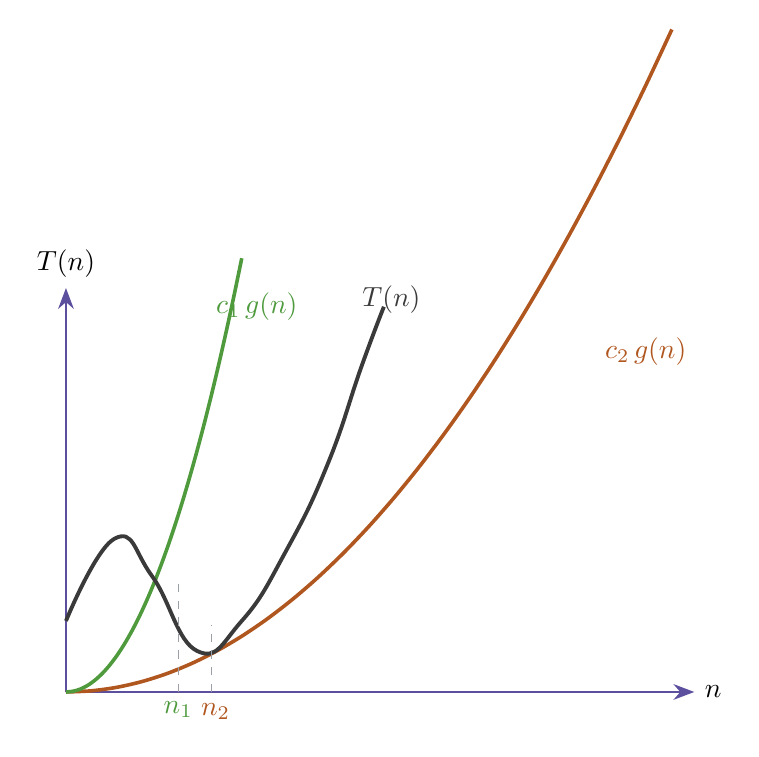
\begin{tikzpicture}[>=Stealth,scale=0.95]
  \draw[violetT,->,line width=1pt] (0,0) -- (0,5.4) node[above,black] {$T(n)$};
  \draw[violetT,->,line width=1pt] (0,0) -- (8.4,0) node[right,black] {$n$};
  \draw[rustW,line width=1.3pt,domain=0:8.1,smooth,variable=\x]
        plot ({\x},{0.135*\x*\x});
  \node[rustW] at (7.75,4.55) {$c_2\, g(n)$};
  \draw[greenO,line width=1.3pt,domain=0:2.35,smooth,variable=\x]
        plot ({\x},{1.05*\x*\x});
  \node[greenO] at (2.55,5.15) {$c_1\, g(n)$};
  \draw[inkT,line width=1.4pt,smooth,tension=0.8]
        plot coordinates {(0,0.95)(0.65,2.05)(1.15,1.55)(1.75,0.55)
                          (2.35,0.95)(2.95,1.9)(3.5,3.05)(3.95,4.35)(4.25,5.15)};
  \node[inkT] at (4.35,5.25) {$T(n)$};
  \draw[greyline,dashed] (1.5,0) -- (1.5,1.55);
  \draw[greyline,dashed] (1.95,0) -- (1.95,0.9);
  \node[greenO,below] at (1.5,0) {$n_1$};
  \node[rustW,below] at (2.0,-0.02) {$n_2$};
\end{tikzpicture}
\end{center}

Past $n_2$, $T(n)$ is trapped between the \textcolor{rustW}{$c_2 g(n)$} floor and the \textcolor{greenO}{$c_1 g(n)$} ceiling. That is $\Theta$.

% ==================================================================
\section{Worked Example: Bubble Sort is $\Theta(n^2)$}

\begin{codebox}[BubbleSort(A)]
\ttfamily for i = 1 to A.length $-$ 1:\\
\ttfamily \hspace*{2em}for j = A.length downto i + 1:\\
\ttfamily \hspace*{4em}if A[j] < A[j$-$1]: swap A[j] and A[j$-$1]
\end{codebox}

\begin{keybox}[Bubble Sort: $T(n) = \Theta(n^2)$]
\textcolor{greenO}{$O(n^2)$:} For \every{} input, the nested loops do $\sum_{i=1}^{n-1}(n-i) = \frac{n(n-1)}{2}$ comparisons. So $T(n) \le c_1 n^2$.

\textcolor{rustW}{$\Omega(n^2)$:} For \some{} input (reverse-sorted: $[n, n{-}1, \ldots, 1]$), every comparison triggers a swap, doing exactly $\frac{n(n-1)}{2}$ comparisons. So $T(n) \ge c_2 n^2$.

Same shape $\Rightarrow$ $\Theta(n^2)$.
\end{keybox}

\begin{examplebox}[Practice: is $3n^2 + 5n\log n$ in $\Theta(n^2)$?]
\textcolor{greenO}{$O(n^2)$:} $3n^2 + 5n\log n \le 3n^2 + 5n^2 = 8n^2$ for $n \ge 1$. \checkmark

\textcolor{rustW}{$\Omega(n^2)$:} $3n^2 + 5n\log n \ge 3n^2$ for $n \ge 1$. \checkmark

Yes, $3n^2 + 5n\log n = \Theta(n^2)$.
\end{examplebox}

\begin{keybox}[Quick Reference: Lecture 1]
\renewcommand{\arraystretch}{1.35}
\begin{tabular}{l l}
$T(n)$ & $\max\{t(x) \mid x \text{ of size } n\}$ \\
\textcolor{greenO}{$O(g(n))$} & $T(n) \le c\,g(n)$ eventually \quad \every{} input, \atmost \\
\textcolor{rustW}{$\Omega(g(n))$} & $T(n) \ge c\,g(n)$ eventually \quad \some{} input, \atleast \\
\textcolor{violetT}{$\Theta(g(n))$} & both $O$ and $\Omega$ with same $g$ (tight) \\
Bubble sort & $\Theta(n^2)$ \\
\end{tabular}
\end{keybox}

\newpage

% ******************************************************************
%  PART II: LECTURE 2 — PRIORITY QUEUES AND MAX-HEAPS
% ******************************************************************

\part*{\textcolor{utnavy}{Lecture 2: Priority Queues and Max-Heaps}}
\addcontentsline{toc}{part}{Lecture 2: Priority Queues and Max-Heaps}

% ==================================================================
\section{ADT vs.\ Data Structure}

\begin{defbox}[Two different things]
\textbf{Abstract data type (ADT):} specifies an \textcolor{rustW}{object} + \textcolor{rustW}{operations}. Says \emph{what}, not \emph{how}.

\textbf{Data structure:} \textcolor{rustW}{one specific implementation} of an ADT (memory layout + code for each operation).

Multiple data structures can implement the same ADT, with different costs.
\end{defbox}

% ==================================================================
\section{The Priority Queue ADT}

\begin{defbox}[Priority Queue ADT]
\textbf{Object:} a set $S$ of elements, each with a comparable \textcolor{rustW}{key} (priority).

\textbf{Operations:}
\begin{itemize}[leftmargin=1.4em,itemsep=1pt]
  \item \textbf{Insert}$(S,x)$: add element $x$ into $S$.
  \item \textbf{Max}$(S)$: return element with highest priority (no removal).
  \item \textbf{Extract\_Max}$(S)$: return \textbf{and remove} element with highest priority.
\end{itemize}
\end{defbox}

\textbf{Application:} OS job scheduling. Jobs arrive $\to$ \textbf{Insert}. Processor free $\to$ \textbf{Extract\_Max} to run the highest-priority job.

% ==================================================================
\section{Naive Implementations: Why We Need Something Better}

\begin{center}
\renewcommand{\arraystretch}{1.5}
\begin{tabular}{l c c}
\hline
\textbf{\textcolor{heapblue}{Worst case}} & \textbf{Insert} & \textbf{Extract\_Max}\\
\hline
Unordered linked list & \textcolor{greenO}{$\Theta(1)$} & \textcolor{rustW}{$\Theta(n)$}\\
Ordered linked list   & \textcolor{rustW}{$\Theta(n)$} & \textcolor{greenO}{$\Theta(1)$}\\
\hline
\end{tabular}
\end{center}

\textbf{Unordered:} Insert at front is $\Theta(1)$, but Extract\_Max scans the whole list $\Rightarrow$ $\Theta(n)$.

\textbf{Ordered:} Max is at the end $\Rightarrow$ Extract\_Max is $\Theta(1)$, but inserting in sorted position $\Rightarrow$ $\Theta(n)$.

\begin{keybox}[Goal]
Both operations in \textcolor{rustW}{$O(\log n)$}. A \textbf{max-heap} achieves this.
\end{keybox}

% ==================================================================
\section{Complete Binary Tree (CBT)}

\begin{defbox}[Complete Binary Tree]
A binary tree where:
\begin{itemize}[leftmargin=1.4em,itemsep=1pt]
  \item every level except possibly the last is completely full,
  \item the last level is filled \textcolor{rustW}{from the left} with no gaps.
\end{itemize}
\end{defbox}

\begin{center}
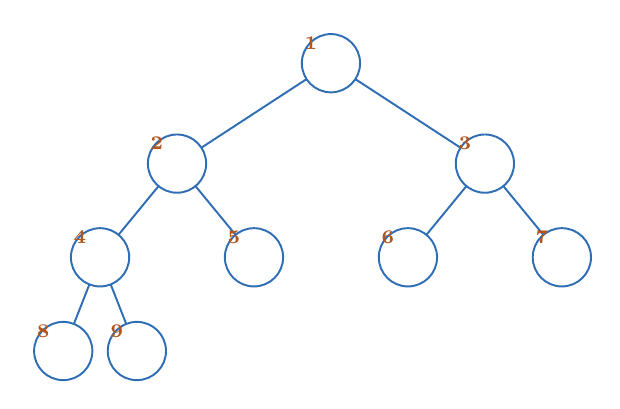
\begin{tikzpicture}[scale=0.85]
\drawheap{1//black,2//black,3//black,4//black,5//black,6//black,7//black,8//black,9//black}{1/2,1/3,2/4,2/5,3/6,3/7,4/8,4/9}
\end{tikzpicture}
\end{center}

\subsection{Height}

\begin{defbox}[Height of a tree]
Number of \textcolor{rustW}{edges} on the longest root-to-leaf path.
\end{defbox}

\begin{center}
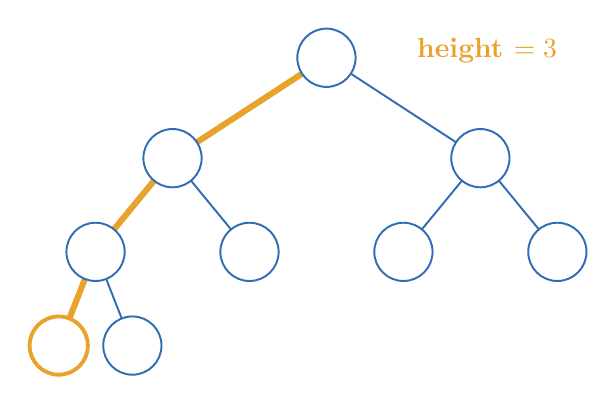
\begin{tikzpicture}[scale=0.85]
\heapcoords
\begin{scope}[on background layer]
  \foreach \a/\b in {1/3,2/5,3/6,3/7,4/9}{\draw[hedge] (p\a)--(p\b);}
  \foreach \a/\b in {1/2,2/4,4/8}{\draw[goldpath,line width=2.2pt] (p\a)--(p\b);}
\end{scope}
\foreach \idx in {1,2,3,4,5,6,7,9}{\node[hnode] at (p\idx){};}
\node[hnode,draw=goldpath,line width=1.4pt] at (p8){};
\node[goldpath,font=\bfseries] at (2.4,4.6){height $=3$};
\end{tikzpicture}
\end{center}

\begin{keybox}[Key fact]
A CBT with $n$ nodes has height $\lfloor \log_2 n \rfloor$.

Each full level doubles the node count ($1, 2, 4, 8, \ldots$), so $\log_2 n$ levels suffice for $n$ nodes.
\end{keybox}

% ==================================================================
\section{Max-Heap}

\begin{defbox}[Max-Heap = CBT + max-heap property]
Elements stored in a CBT such that:
\begin{center}\large
priority(node) $\;\textcolor{rustW}{\ge}\;$ priority(each child)
\end{center}
This is a \textbf{local} rule (parent vs.\ own children only). It chains upward, so the \textbf{global max is always at the root}.
\end{defbox}

\subsection*{Example}
$S=\{3,4,5,7,7,9,9,12,17\}$. One valid max-heap:

\begin{center}
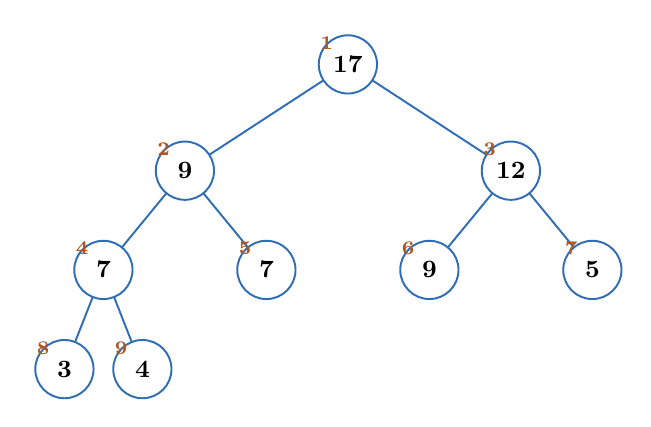
\begin{tikzpicture}[scale=0.9]
\drawheap{1/17/black,2/9/black,3/12/black,4/7/black,5/7/black,6/9/black,7/5/black,8/3/black,9/4/black}{1/2,1/3,2/4,2/5,3/6,3/7,4/8,4/9}
\end{tikzpicture}
\end{center}

Check: $17 \ge 9, 12$. \; $9 \ge 7, 7$. \; $12 \ge 9, 5$. \checkmark

Swapping children of the root ($9 \leftrightarrow 12$) gives a different valid heap $\Rightarrow$ \textcolor{rustW}{max-heaps are not unique}. Only the root (global max) is guaranteed.

% ==================================================================
\section{Array Representation}

Store the tree \textbf{level by level, left to right} in array \texttt{A[1..n]}. No pointers needed.

\begin{center}
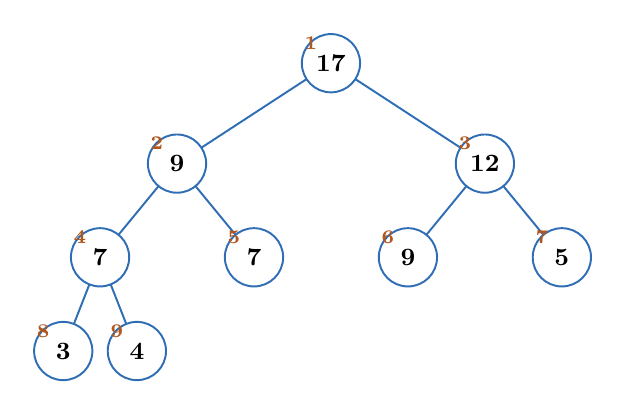
\begin{tikzpicture}[scale=0.85]
\drawheap{1/17/black,2/9/black,3/12/black,4/7/black,5/7/black,6/9/black,7/5/black,8/3/black,9/4/black}{1/2,1/3,2/4,2/5,3/6,3/7,4/8,4/9}
\end{tikzpicture}\\[8pt]
\heaparray{17,9,12,7,7,9,5,3,4}
\end{center}

\begin{keybox}[Navigation formulas]
For node at index $i$:
\begin{itemize}[leftmargin=1.4em,itemsep=1pt]
  \item \textbf{Left child:} $2i$ \qquad \textbf{Right child:} $2i+1$ \qquad \textbf{Parent:} $\lfloor i/2 \rfloor$
\end{itemize}
\texttt{A.heapsize} tracks the number of elements currently in the heap.
\end{keybox}

\begin{examplebox}[Verify: node at $i=2$ holds $9$]
Left child: $A[2 \cdot 2] = A[4] = 7$ \checkmark \quad Right child: $A[2 \cdot 2 + 1] = A[5] = 7$ \checkmark

Parent: $A[\lfloor 2/2 \rfloor] = A[1] = 17$ \checkmark

Each level is $\sim 2\times$ the width of the one above, so going down doubles the index, going up halves it.
\end{examplebox}

% ==================================================================
\section{The Three Operations}

\begin{keybox}[Invariant for every operation]
1) Maintain the \textcolor{rustW}{CBT shape}. \quad 2) Maintain the \textcolor{rustW}{max-heap property}.
\end{keybox}

\subsection{Max(A)}

\begin{codebox}[Max(A)]
\ttfamily return A[1]
\end{codebox}

The root always holds the max. $\Rightarrow$ \textcolor{greenO}{$\Theta(1)$}.

\subsection{Insert(A, x): percolate up}

\begin{codebox}[Insert(A, x)]
\ttfamily 1. A.heapsize++; A[A.heapsize] = x \hfill\textnormal{\itshape (place at next open leaf)}\\[3pt]
\ttfamily 2. while x is not root and priority(x) > priority(parent(x)):\\
\ttfamily \hspace*{2em}swap x with parent(x) \hfill\textnormal{\itshape (percolate up)}
\end{codebox}

\subsubsection*{Worked example: Insert(A, 13)}
Start: $A = [17,9,12,7,7,9,5,3,4]$. Insert $13$ at index $10$.

\textbf{Step 1.} Place $13$ at $A[10]$. Property broken: $13 > 7$ (parent at $i=5$).

\begin{center}
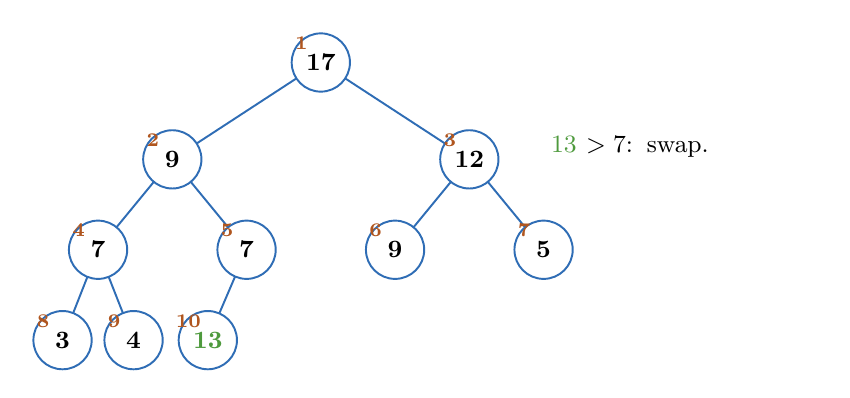
\begin{tikzpicture}[scale=0.82]
\drawheap{1/17/black,2/9/black,3/12/black,4/7/black,5/7/black,6/9/black,7/5/black,8/3/black,9/4/black,10/13/greenO}{1/2,1/3,2/4,2/5,3/6,3/7,4/8,4/9,5/10}
\node[align=left,text width=3.3cm] at (5.6,3.2){\small \textcolor{greenO}{$13$} $> 7$: swap.};
\end{tikzpicture}
\end{center}

\textbf{Step 2a.} Swap $13 \leftrightarrow 7$. Now $13$ at $i=5$. Compare: $13 > 9$ (parent at $i=2$).

\begin{center}
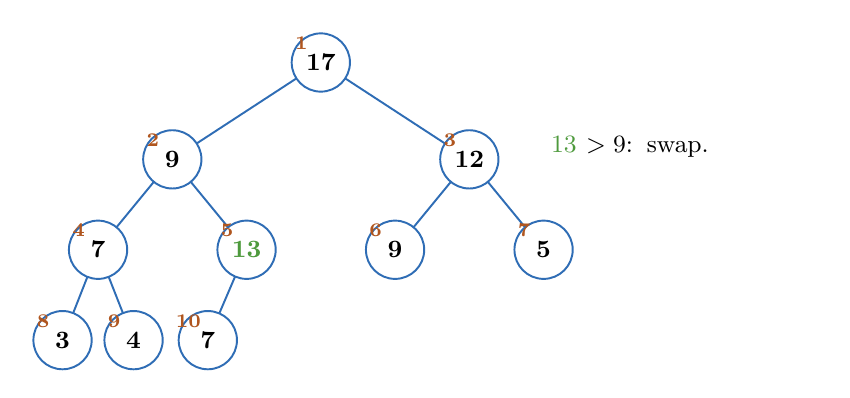
\begin{tikzpicture}[scale=0.82]
\drawheap{1/17/black,2/9/black,3/12/black,4/7/black,5/13/greenO,6/9/black,7/5/black,8/3/black,9/4/black,10/7/black}{1/2,1/3,2/4,2/5,3/6,3/7,4/8,4/9,5/10}
\node[align=left,text width=3.3cm] at (5.6,3.2){\small \textcolor{greenO}{$13$} $> 9$: swap.};
\end{tikzpicture}
\end{center}

\textbf{Step 2b.} Swap $13 \leftrightarrow 9$. Now $13$ at $i=2$. Compare: $13 < 17$ (root). Stop.

\begin{center}
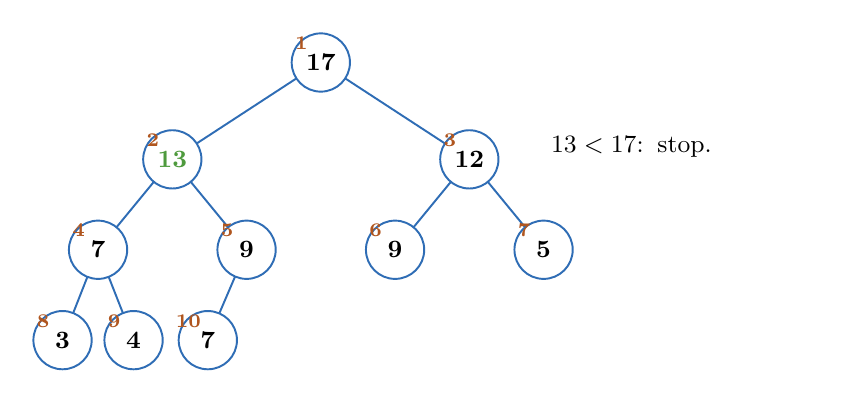
\begin{tikzpicture}[scale=0.82]
\drawheap{1/17/black,2/13/greenO,3/12/black,4/7/black,5/9/black,6/9/black,7/5/black,8/3/black,9/4/black,10/7/black}{1/2,1/3,2/4,2/5,3/6,3/7,4/8,4/9,5/10}
\node[align=left,text width=3.3cm] at (5.6,3.2){\small $13 < 17$: stop.};
\end{tikzpicture}
\end{center}

Result: $A = [17,13,12,7,9,9,5,3,4,7]$, \texttt{heapsize}$=10$.

\subsection{Extract\_Max(A): drip down}

\begin{codebox}[Extract\_Max(A)]
\ttfamily 1. max = A[1] \hfill\textnormal{\itshape (save the root)}\\[3pt]
\ttfamily 2. A[1] = A[A.heapsize]; A.heapsize{-}{-} \hfill\textnormal{\itshape (move last leaf to root)}\\[3pt]
\ttfamily 3. while x has a child with higher priority:\\
\ttfamily \hspace*{2em}swap x with its \textbf{largest} child \hfill\textnormal{\itshape (drip down)}\\[3pt]
\ttfamily 4. return max
\end{codebox}

Important: always swap with the \emph{larger} child (otherwise we create a new violation). Node at index $i$ is a leaf when $i > \lfloor \texttt{heapsize}/2 \rfloor$.

\subsubsection*{Worked example: Extract\_Max(A)}
Start: $A = [17,13,12,7,9,9,5,3,4,7]$, \texttt{heapsize}$=10$.

\textbf{Steps 1\,\&\,2.} Save $17$. Move $A[10]=7$ to root. Shrink \texttt{heapsize} to $9$.

\begin{center}
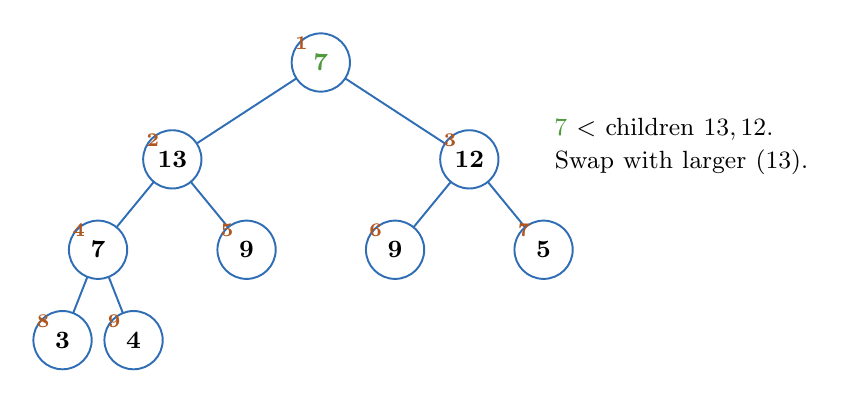
\begin{tikzpicture}[scale=0.82]
\drawheap{1/7/greenO,2/13/black,3/12/black,4/7/black,5/9/black,6/9/black,7/5/black,8/3/black,9/4/black}{1/2,1/3,2/4,2/5,3/6,3/7,4/8,4/9}
\node[align=left,text width=3.4cm] at (5.7,3.2){\small \textcolor{greenO}{$7$} $<$ children $13, 12$. Swap with larger ($13$).};
\end{tikzpicture}
\end{center}

\textbf{Step 3a.} Swap $7 \leftrightarrow 13$. Now $7$ at $i=2$. Children: $7, 9$. Larger is $9 > 7$.

\begin{center}
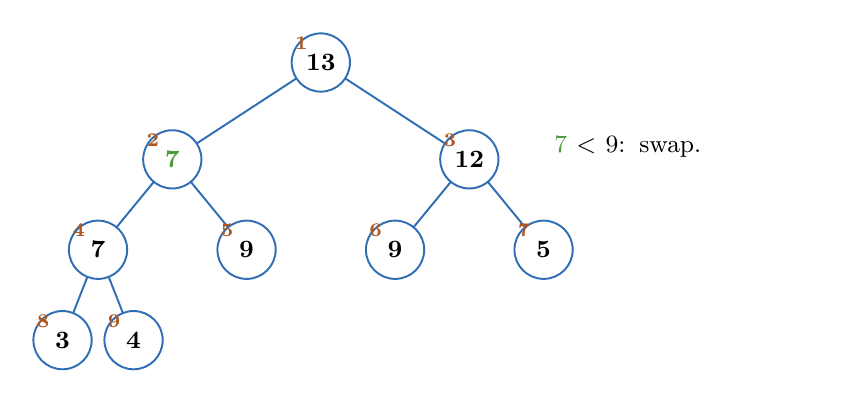
\begin{tikzpicture}[scale=0.82]
\drawheap{1/13/black,2/7/greenO,3/12/black,4/7/black,5/9/black,6/9/black,7/5/black,8/3/black,9/4/black}{1/2,1/3,2/4,2/5,3/6,3/7,4/8,4/9}
\node[align=left,text width=3.4cm] at (5.7,3.2){\small \textcolor{greenO}{$7$} $<$ $9$: swap.};
\end{tikzpicture}
\end{center}

\textbf{Step 3b.} Swap $7 \leftrightarrow 9$. Now $7$ at $i=5$. Children at $i=10 >$ \texttt{heapsize}$=9$, so $7$ is a leaf. Stop.

\begin{center}
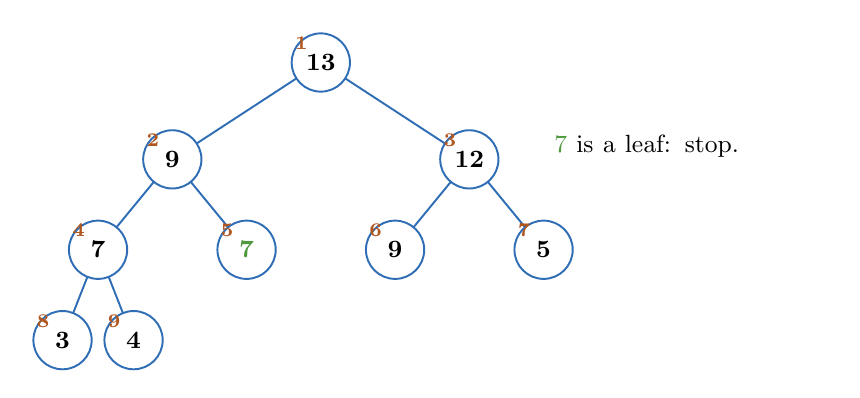
\begin{tikzpicture}[scale=0.82]
\drawheap{1/13/black,2/9/black,3/12/black,4/7/black,5/7/greenO,6/9/black,7/5/black,8/3/black,9/4/black}{1/2,1/3,2/4,2/5,3/6,3/7,4/8,4/9}
\node[align=left,text width=3.4cm] at (5.7,3.2){\small \textcolor{greenO}{$7$} is a leaf: stop.};
\end{tikzpicture}
\end{center}

Return $17$. Heap: $[13,9,12,7,7,9,5,3,4]$.

% ==================================================================
\section{Complexity Analysis}

Each operation walks one root-to-leaf (or leaf-to-root) path. Path length $\le$ height $= \lfloor \log_2 n \rfloor$. Constant work per level.

\begin{keybox}[Heap operation costs]
\renewcommand{\arraystretch}{1.4}
\begin{tabular}{l l l}
\textbf{Max}$(A)$ & \textcolor{greenO}{$\Theta(1)$} & read root\\
\textbf{Insert}$(A,x)$ & \textcolor{violetT}{$\Theta(\log n)$} & percolate up $\le \lfloor\log_2 n\rfloor$ levels\\
\textbf{Extract\_Max}$(A)$ & \textcolor{violetT}{$\Theta(\log n)$} & drip down $\le \lfloor\log_2 n\rfloor$ levels\\
\end{tabular}
\end{keybox}

\textbf{Insert} $= \Theta(\log n)$:
\begin{itemize}[leftmargin=1.4em,itemsep=2pt]
  \item \textcolor{greenO}{$O(\log n)$:} At most $\lfloor\log_2 n\rfloor$ swaps (one per level). \every{} input, \atmost{} $c_1 \log n$.
  \item \textcolor{rustW}{$\Omega(\log n)$:} Insert a value larger than the current root $\Rightarrow$ percolates all the way to the top. \some{} input, \atleast{} $c_2 \log n$.
\end{itemize}

Same argument for Extract\_Max (drip down with the smallest value $\Rightarrow$ sinks to a leaf).

% ==================================================================
\section{HeapSort}

\begin{keybox}[HeapSort]
\begin{enumerate}[leftmargin=1.6em,itemsep=2pt]
  \item Build a max-heap from $A$. \quad{\small($\Theta(n)$ time)}
  \item Call \textbf{Extract\_Max} $n$ times. \quad{\small(each $\Theta(\log n)$)}
\end{enumerate}
\[
  \text{Total: } n \times \Theta(\log n) = \textcolor{violetT}{\Theta(n \log n)}
\]
\end{keybox}

\begin{center}
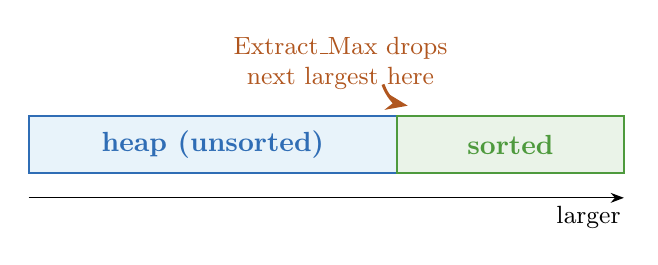
\begin{tikzpicture}[scale=0.9]
\draw[fill=skyfill,draw=heapblue,line width=0.7pt] (0,0) rectangle (5.2,0.8);
\draw[fill=greenO!12,draw=greenO,line width=0.7pt] (5.2,0) rectangle (8.4,0.8);
\node[heapblue,font=\bfseries] at (2.6,0.4){heap (unsorted)};
\node[greenO,font=\bfseries] at (6.8,0.4){sorted};
\draw[-{Stealth},line width=1.1pt,rustW] (5.0,1.25) to[bend right=30] (5.35,0.95);
\node[rustW,font=\small,align=center] at (4.4,1.55){Extract\_Max drops\\next largest here};
\draw[-{Stealth}] (0,-0.35)--(8.4,-0.35);
\node[font=\small] at (7.9,-0.62){larger};
\end{tikzpicture}
\end{center}

Each extraction moves the max to the front of the sorted region. The heap shrinks by one, the sorted region grows by one. After $n$ extractions, the array is sorted in place.

% ==================================================================
\section{Past Exam: $k$-Set ADT}

\begin{exambox}[Seen on a past exam \textnormal{(Midterm, Fall 2014, Q2)}]
The \emph{rank} of an element = its position in sorted order (from $1$). For fixed $k \in \mathbb{Z}^+$:
\begin{itemize}[leftmargin=1.4em,itemsep=1pt]
  \item \textbf{Object:} collection $C$ of rationals (duplicates allowed).
  \item \textbf{Insert}$(C,x)$: add $x$ to $C$.
  \item \textbf{$k$-Select}$(C)$: return element at rank $k$, or \texttt{nil} if $|C| < k$.
\end{itemize}
\textbf{Q.} Implement with data structures from class. \textbf{$k$-Select} must be $O(1)$.

\begin{answerband}
\textbf{Data structure:} \textbf{max-heap} $H_1$ (stores the $k$ smallest elements) + \textbf{min-heap} $H_2$ (stores the rest).

The $k$-th smallest element = the largest among the $k$ smallest = root of $H_1$.

\smallskip
\textbf{$k$-Select$(C)$:}\\
\hspace*{1.5em}\texttt{if $|H_1| < k$: return nil}\\
\hspace*{1.5em}\texttt{else: return $H_1[1]$} \hfill $\Rightarrow$ \textcolor{greenO}{$O(1)$}

\smallskip
\textbf{Insert$(C,x)$:}\\
\hspace*{1.5em}\texttt{if $|H_1| < k$ or $x < H_1[1]$: insert $x$ into $H_1$}\\
\hspace*{1.5em}\texttt{else: insert $x$ into $H_2$}\\
\hspace*{1.5em}\texttt{if $|H_1| > k$: insert Extract-Max($H_1$) into $H_2$}\\
Constant number of heap ops, each $O(\log n)$ $\Rightarrow$ \textcolor{violetT}{$O(\log n)$}.

\smallskip
\textbf{Correctness:} $H_1$ always holds exactly the $k$ smallest. New small values enter $H_1$; overflow gets pushed to $H_2$. Large values go straight to $H_2$.
\end{answerband}
\end{exambox}

% ==================================================================
\section*{\textcolor{violetT}{Quick Reference: Lecture 2}}
\addcontentsline{toc}{section}{Quick Reference: Lecture 2}
\begin{keybox}
\renewcommand{\arraystretch}{1.35}
\begin{tabular}{l l}
Max-heap property & priority(node) $\ge$ priority(children); max at root \texttt{A[1]}\\
Array navigation & left $=2i$, \; right $=2i+1$, \; parent $=\lfloor i/2\rfloor$\\
Height of CBT & $\lfloor \log_2 n \rfloor$\\
\textbf{Max} & read \texttt{A[1]} $\to$ \textcolor{greenO}{$\Theta(1)$}\\
\textbf{Insert} & place at end, percolate up $\to$ \textcolor{violetT}{$\Theta(\log n)$}\\
\textbf{Extract\_Max} & move last to root, drip down $\to$ \textcolor{violetT}{$\Theta(\log n)$}\\
\textbf{HeapSort} & build heap + $n$ extractions $\to$ \textcolor{violetT}{$\Theta(n\log n)$}\\
\end{tabular}
\end{keybox}

\vspace{4pt}
\begin{center}\textcolor{greyline}{\rule{0.5\linewidth}{0.6pt}}\end{center}
\begin{center}\small\textcolor{greyline}{End of Lectures 1 \& 2 notes.}\end{center}


\newpage
 


% ******************************************************************
%  PASTE INSTRUCTIONS:
%
%  1. In your master document, DELETE these 3 lines near the end:
%       \begin{center}\textcolor{greyline}{\rule{0.5\linewidth}{0.6pt}}\end{center}
%       \begin{center}\small\textcolor{greyline}{End of Lectures 1 \& 2 notes.}\end{center}
%       \end{document}
%
%  2. Paste EVERYTHING below this comment block in their place.
%
%  3. On the cover page, change:
%       {\large\textcolor{violetT}{Lectures 1 \& 2}}
%     to:
%       {\large\textcolor{violetT}{Lectures 1, 2 \& 3}}
%
%  That's it. No preamble changes needed.
% ******************************************************************

\newpage

% ******************************************************************
%  PART III: LECTURE 3 — MIN BINOMIAL HEAPS
% ******************************************************************

\part*{\textcolor{utnavy}{Lecture 3: Min Binomial Heaps}}
\addcontentsline{toc}{part}{Lecture 3: Min Binomial Heaps}

% ==================================================================
\section{Mergeable Priority Queue ADT}

Last lecture: Priority Queue ADT (Insert, Max, Extract\_Max). Now we flip to \textbf{min} (smallest key = highest priority) and add one more operation:

\begin{defbox}[Mergeable Priority Queue ADT]
\textbf{Object:} a set $S$ of elements, each with a comparable \textcolor{rustW}{key}.

\textbf{Operations:}
\begin{itemize}[leftmargin=1.4em,itemsep=1pt]
  \item \textbf{Insert}$(S, x)$: add element $x$ to $S$.
  \item \textbf{Min}$(S)$: return the element with the smallest key.
  \item \textbf{Extract\_Min}$(S)$: remove and return the element with the smallest key.
  \item \textbf{Union}$(S_1, S_2)$: merge two priority queues into a single one.
\end{itemize}
\end{defbox}

\begin{center}
\renewcommand{\arraystretch}{1.5}
\begin{tabular}{l c c}
\hline
\textbf{\textcolor{heapblue}{Operation}} & \textbf{Min Heap (array)} & \textbf{Min Binomial Heap}\\
\hline
\texttt{Insert} & $O(\log n)$ & $O(\log n)$\\
\texttt{Min} & \textcolor{greenO}{$O(1)$} & $O(\log n)$\\
\texttt{Extract\_Min} & $O(\log n)$ & $O(\log n)$\\
\texttt{Union} & \textcolor{rustW}{$O(n)$} & \textcolor{greenO}{$O(\log n)$}\\
\hline
\end{tabular}
\end{center}

\begin{warnbox}[Why regular min heaps fail at Union]
A binary min heap stores elements in an array. To merge two heaps you basically dump them together and rebuild. That costs $O(n)$. Binomial heaps are specifically \textbf{designed} so Union runs in $\textcolor{greenO}{O(\log n)}$.
\end{warnbox}

% ==================================================================
\section{Binomial Trees}

\subsection{Recursive Definition of $B_k$}

\begin{defbox}[Binomial Tree $B_k$]
\textbf{Base case:} $B_0$ = a single node.\\[4pt]
\textbf{Recursive case:} $B_k$ = take two copies of $B_{k-1}$. Make one root the \textbf{leftmost child} of the other root.\\[6pt]
Equivalently: the root of $B_k$ has children $B_{k-1},\, B_{k-2},\, \ldots,\, B_1,\, B_0$ (left to right).
\end{defbox}

\begin{keybox}[Breaking Down the Recursive Definition]
This is a common confusion point, so let's be explicit.

To build $B_k$:
\begin{enumerate}[leftmargin=1.4em,itemsep=2pt]
  \item Start with one copy of $B_{k-1}$. Call its root $r$.
  \item Take a \textbf{second} copy of $B_{k-1}$.
  \item Make the root of copy 2 the \textbf{new overall root}, and attach $r$'s entire tree as a subtree under it.
\end{enumerate}

So $B_k$ = \textbf{two $B_{k-1}$'s glued together}, one becoming a child of the other.
\end{keybox}

\subsubsection*{Building Up From $B_0$}

\begin{center}
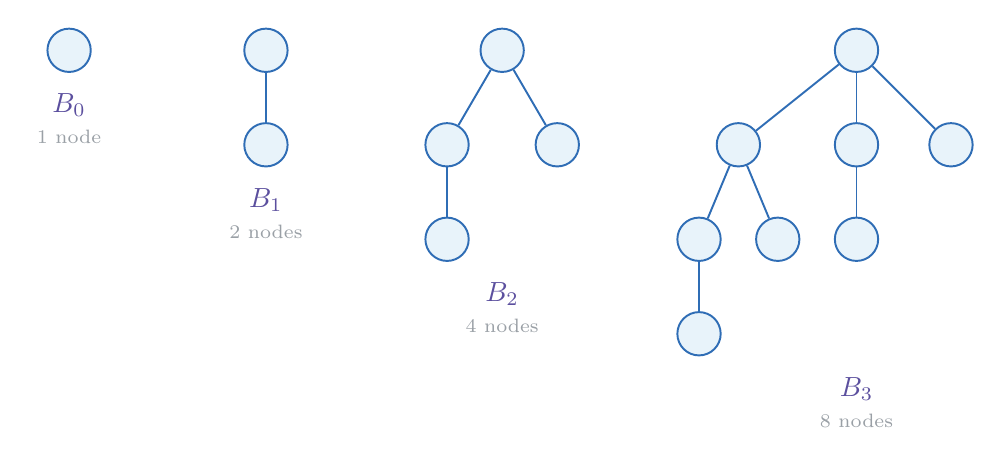
\begin{tikzpicture}[
  bnode/.style={circle, draw=heapblue, line width=0.7pt, minimum size=5.5mm, inner sep=0pt, fill=skyfill},
]
% B_0
\node[bnode] (a0) at (0,0) {};
\node[font=\bfseries\color{violetT}] at (0,-0.7) {$B_0$};
\node[font=\scriptsize\color{greyline}] at (0,-1.1) {1 node};

% B_1
\node[bnode] (b0) at (2.5,0) {};
\node[bnode] (b1) at (2.5,-1.2) {};
\draw[heapblue, line width=0.7pt] (b0) -- (b1);
\node[font=\bfseries\color{violetT}] at (2.5,-1.9) {$B_1$};
\node[font=\scriptsize\color{greyline}] at (2.5,-2.3) {2 nodes};

% B_2
\node[bnode] (c0) at (5.5,0) {};
\node[bnode] (c1) at (4.8,-1.2) {};
\node[bnode] (c2) at (6.2,-1.2) {};
\node[bnode] (c3) at (4.8,-2.4) {};
\draw[heapblue, line width=0.7pt] (c0) -- (c1);
\draw[heapblue, line width=0.7pt] (c0) -- (c2);
\draw[heapblue, line width=0.7pt] (c1) -- (c3);
\node[font=\bfseries\color{violetT}] at (5.5,-3.1) {$B_2$};
\node[font=\scriptsize\color{greyline}] at (5.5,-3.5) {4 nodes};

% B_3
\node[bnode] (d0) at (10,0) {};
\node[bnode] (d1) at (8.5,-1.2) {};
\node[bnode] (d2) at (10,-1.2) {};
\node[bnode] (d3) at (11.2,-1.2) {};
\node[bnode] (d4) at (8,-2.4) {};
\node[bnode] (d5) at (9,-2.4) {};
\node[bnode] (d6) at (10,-2.4) {};
\node[bnode] (d7) at (8,-3.6) {};
\draw[heapblue, line width=0.7pt] (d0) -- (d1);
\draw[heapblue, line width=0.7pt] (d0) -- (d2);
\draw[heapblue, line width=0.7pt] (d0) -- (d3);
\draw[heapblue, line width=0.7pt] (d1) -- (d4);
\draw[heapblue, line width=0.7pt] (d1) -- (d5);
\draw[heapblue, line width=0.7pt] (d2) -- (d6);
\draw[heapblue, line width=0.7pt] (d4) -- (d7);
\node[font=\bfseries\color{violetT}] at (10,-4.3) {$B_3$};
\node[font=\scriptsize\color{greyline}] at (10,-4.7) {8 nodes};
\end{tikzpicture}
\end{center}

\subsection{Children Sequence of $B_k$}

\begin{keybox}[Children of the Root of $B_k$]
The root of $B_k$ has exactly $k$ children. Reading \textbf{left to right}:
$$\underbrace{B_{k-1}}_{\text{leftmost (biggest)}},\; B_{k-2},\; \ldots,\; B_1,\; \underbrace{B_0}_{\text{rightmost (single node)}}$$

The \textcolor{rustW}{leftmost} child is the \textcolor{rustW}{largest} subtree ($B_{k-1}$), and the \textcolor{greenO}{rightmost} child is the \textcolor{greenO}{smallest} ($B_0$).

This ordering matters a lot for the memory representation later.
\end{keybox}

\begin{examplebox}[Visualizing $B_4$: Children of the Root]
The \textcolor{rustW}{root} of $B_4$ has children $B_3, B_2, B_1, B_0$ (left to right, largest subtree to smallest). Total: $2^4 = 16$ nodes, height 4.

\begin{center}
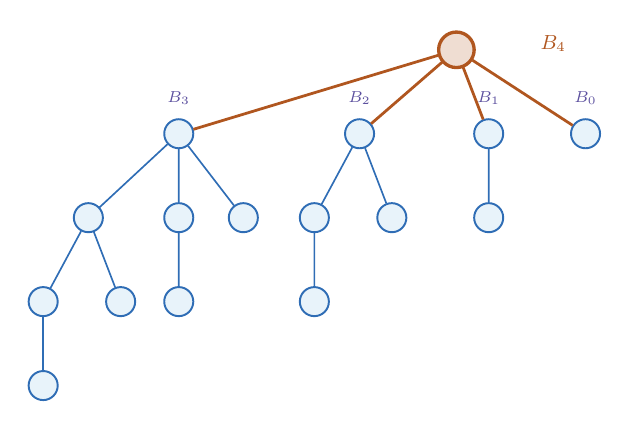
\begin{tikzpicture}[
  bnode/.style={circle, draw=heapblue, line width=0.7pt, minimum size=4.5mm, inner sep=0pt, fill=skyfill},
  rnode/.style={circle, draw=rustW, line width=1.2pt, minimum size=5.5mm, inner sep=0pt, fill=rustW!20},
  scale=0.82, transform shape
]
% Level 0 (root)
\node[rnode] (r) at (5.5,0) {};
\node[font=\small\bfseries\color{rustW}] at (7,0.1) {$B_4$};

% Level 1: 4 children
\node[bnode] (a) at (1.2,-1.3) {};
\node[bnode] (b) at (4,-1.3) {};
\node[bnode] (c) at (6,-1.3) {};
\node[bnode] (d) at (7.5,-1.3) {};
\draw[rustW, line width=1pt] (r)--(a); \draw[rustW, line width=1pt] (r)--(b);
\draw[rustW, line width=1pt] (r)--(c); \draw[rustW, line width=1pt] (r)--(d);

% B_3 subtree (under a): 3 children
\node[bnode] (a1) at (-0.2,-2.6) {};
\node[bnode] (a2) at (1.2,-2.6) {};
\node[bnode] (a3) at (2.2,-2.6) {};
\draw[heapblue,line width=0.6pt] (a)--(a1); \draw[heapblue,line width=0.6pt] (a)--(a2);
\draw[heapblue,line width=0.6pt] (a)--(a3);
% Level 3 of B_3
\node[bnode] (a11) at (-0.9,-3.9) {};
\node[bnode] (a12) at (0.3,-3.9) {};
\node[bnode] (a21) at (1.2,-3.9) {};
\draw[heapblue,line width=0.6pt] (a1)--(a11); \draw[heapblue,line width=0.6pt] (a1)--(a12);
\draw[heapblue,line width=0.6pt] (a2)--(a21);
% Level 4 of B_3
\node[bnode] (a111) at (-0.9,-5.2) {};
\draw[heapblue,line width=0.6pt] (a11)--(a111);

% B_2 subtree (under b): 2 children
\node[bnode] (b1) at (3.3,-2.6) {};
\node[bnode] (b2) at (4.5,-2.6) {};
\draw[heapblue,line width=0.6pt] (b)--(b1); \draw[heapblue,line width=0.6pt] (b)--(b2);
\node[bnode] (b11) at (3.3,-3.9) {};
\draw[heapblue,line width=0.6pt] (b1)--(b11);

% B_1 subtree (under c): 1 child
\node[bnode] (c1) at (6,-2.6) {};
\draw[heapblue,line width=0.6pt] (c)--(c1);

% Subtree labels
\node[font=\scriptsize\bfseries\color{violetT}] at (1.2,-0.75) {$B_3$};
\node[font=\scriptsize\bfseries\color{violetT}] at (4,-0.75) {$B_2$};
\node[font=\scriptsize\bfseries\color{violetT}] at (6,-0.75) {$B_1$};
\node[font=\scriptsize\bfseries\color{violetT}] at (7.5,-0.75) {$B_0$};
\end{tikzpicture}
\end{center}
\end{examplebox}

\subsection{Properties of $B_k$}

\begin{keybox}[Key Properties of $B_k$]
\renewcommand{\arraystretch}{1.5}
\begin{tabular}{l l}
\textbf{\textcolor{violetT}{Height}} of $B_k$ & $= k$ \\
\textbf{\textcolor{violetT}{Number of nodes}} in $B_k$ & $= 2^k$ \\
\textbf{\textcolor{violetT}{Nodes at depth $d$}} in $B_k$ & $= \displaystyle\binom{k}{d}$ \\
\textbf{\textcolor{violetT}{Degree}} of root of $B_k$ & $= k$ \\
\end{tabular}
\end{keybox}

\subsection{Why ``Binomial''?}

\begin{examplebox}[Why the Name ``Binomial'']
The number of nodes at depth $d$ in $B_k$ is $\binom{k}{d}$, the \textbf{binomial coefficient} (same ``$n$ choose $k$'' from combinatorics).

Quick check for $B_3$ (8 nodes total):

\begin{center}
\renewcommand{\arraystretch}{1.3}
\begin{tabular}{l c l}
Depth 0: & $\binom{3}{0} = 1$ & (the root)\\
Depth 1: & $\binom{3}{1} = 3$ & \\
Depth 2: & $\binom{3}{2} = 3$ & \\
Depth 3: & $\binom{3}{3} = 1$ & \\
\end{tabular}
\end{center}
Total: $1 + 3 + 3 + 1 = 8$ \checkmark
\end{examplebox}

% ==================================================================
\section{Binomial Forest $F_n$}

\begin{defbox}[Binomial Forest $F_n$]
A \textbf{Binomial Forest} $F_n$ is a sequence of binomial trees $\langle B_{k_1}, B_{k_2}, \ldots, B_{k_m} \rangle$ where:
\begin{itemize}[leftmargin=1.4em,itemsep=1pt]
  \item The $k_i$ values are \textbf{strictly decreasing}: $k_1 > k_2 > \cdots > k_m$
  \item The total number of nodes across all trees $= n$
\end{itemize}
\end{defbox}

\subsection{Connection to Binary Representation}

\begin{keybox}[Binary Representation $\Leftrightarrow$ Which Trees Are Present]
Write $n$ in binary. $B_i$ is present in $F_n$ \textbf{if and only if} bit $i$ (counting from the right, starting at 0) is \textbf{1}.

This is one of the most important ideas in this lecture. The entire structure of a binomial heap is dictated by the binary representation of $n$.
\end{keybox}

\begin{examplebox}[Example: $F_7$ and $F_9$]
\textbf{$F_7$:} \quad $7 = \langle 111 \rangle_2$

All three bits are 1, so $F_7 = \langle B_2, B_1, B_0 \rangle$.

Sizes: $4 + 2 + 1 = 7$ \checkmark \\[6pt]

\textbf{$F_9$:} \quad $9 = \langle 1001 \rangle_2$

Bits 0 and 3 are 1, so $F_9 = \langle B_3, B_0 \rangle$.

Sizes: $8 + 1 = 9$ \checkmark
\end{examplebox}

\subsection{What is $\alpha(n)$?}

\begin{defbox}[$\alpha(n)$ (popcount)]
$\alpha(n)$ = the number of \textbf{1's} in the binary representation of $n$.

Other names: \textbf{popcount}, \textbf{Hamming weight}, \textbf{bit population count}.
\end{defbox}

\begin{examplebox}[Computing $\alpha(n)$]
\begin{center}
\renewcommand{\arraystretch}{1.3}
\begin{tabular}{l l l}
$\alpha(7)$ & $= \alpha(\langle 111 \rangle_2)$ & $= 3$ \\
$\alpha(9)$ & $= \alpha(\langle 1001 \rangle_2)$ & $= 2$ \\
$\alpha(16)$ & $= \alpha(\langle 10000 \rangle_2)$ & $= 1$ \\
$\alpha(15)$ & $= \alpha(\langle 1111 \rangle_2)$ & $= 4$ \\
\end{tabular}
\end{center}
\end{examplebox}

\subsection{Properties of $F_n$}

\begin{keybox}[Properties of $F_n$]
\renewcommand{\arraystretch}{1.5}
\begin{tabular}{l l}
Number of trees in $F_n$ & $= \textcolor{violetT}{\alpha(n)}$ \quad (one per 1 bit) \\
Max number of trees & $\le \lfloor \log_2 n \rfloor + 1$ \\
Number of edges in $F_n$ & $= \textcolor{violetT}{n - \alpha(n)}$ \\
\end{tabular}
\end{keybox}

\begin{examplebox}[Verifying Edge Count for $F_7$]
$F_7 = \langle B_2, B_1, B_0 \rangle$.

Edges in $B_2$: 3, \quad edges in $B_1$: 1, \quad edges in $B_0$: 0. \quad Total = 4.

Formula: $n - \alpha(n) = 7 - 3 = 4$ \checkmark
\end{examplebox}

% ==================================================================
\section{Min Binomial Heap: The Full Definition}

\begin{defbox}[Min Binomial Heap]
A \textbf{Min Binomial Heap} of $n$ elements is a Binomial Forest $F_n$ such that:
\begin{enumerate}[leftmargin=1.4em,itemsep=3pt]
  \item \textcolor{defblue}{\textbf{One element per node:}} each node stores exactly one element.
  \item \textcolor{defblue}{\textbf{Min heap ordering:}} in each tree, every node's key $\le$ all keys in its subtree. (Root of each tree = smallest key in that tree.)
\end{enumerate}
\end{defbox}

\begin{warnbox}[It's a forest, not a single tree!]
A Min Binomial Heap is a \textbf{collection of trees} (a forest). Each individual tree is a binomial tree satisfying the min heap property. Do not confuse this with a single binary heap.
\end{warnbox}

% ==================================================================
\section{Building a Binomial Heap: Worked Example}

\begin{examplebox}[Build a Min Binomial Heap from $S = \{10, 13, 1, 3, 8, 18, 7\}$]
$n = 7$, and $7 = \langle 111 \rangle_2$, so the final forest = $\langle B_2, B_1, B_0 \rangle$.

\textbf{Insert 10:} $n=1 = \langle 1 \rangle_2 \Rightarrow \langle B_0 \rangle$
\begin{center} $B_0$: \fbox{10} \end{center}

\textbf{Insert 13:} $n=2 = \langle 10 \rangle_2 \Rightarrow \langle B_1 \rangle$

Two $B_0$'s $\to$ merge. Compare 10 vs 13: $10 \le 13$, so 10 is root.
\begin{center} $B_1$: 10 $\to$ 13 \end{center}

\textbf{Insert 1:} $n=3 = \langle 11 \rangle_2 \Rightarrow \langle B_1, B_0 \rangle$

1 sits as the new $B_0$, $B_1$ stays.
\begin{center} $B_1$: 10 $\to$ 13 \qquad $B_0$: \fbox{1} \end{center}

\textbf{Insert 3:} $n=4 = \langle 100 \rangle_2 \Rightarrow \langle B_2 \rangle$

3 forms $B_0$. Two $B_0$'s (1 and 3): $1 \le 3 \Rightarrow B_1$(root 1, child 3). Two $B_1$'s (root 1 vs root 10): $1 \le 10 \Rightarrow B_2$(root 1). \quad \textcolor{rustW}{2 comparisons.}
\begin{center} $B_2$: root 1, children: $B_1$(10$\to$13) and $B_0$(3) \end{center}

\textbf{Insert 8:} $n=5 = \langle 101 \rangle_2 \Rightarrow \langle B_2, B_0 \rangle$
\begin{center} $B_2$(root 1) \qquad $B_0$: \fbox{8} \qquad \textcolor{greenO}{0 comparisons.} \end{center}

\textbf{Insert 18:} $n=6 = \langle 110 \rangle_2 \Rightarrow \langle B_2, B_1 \rangle$

Two $B_0$'s (8 and 18): $8 \le 18 \Rightarrow B_1$(root 8, child 18). \quad \textcolor{rustW}{1 comparison.}
\begin{center} $B_2$(root 1) \qquad $B_1$: 8$\to$18 \end{center}

\textbf{Insert 7:} $n=7 = \langle 111 \rangle_2 \Rightarrow \langle B_2, B_1, B_0 \rangle$

7 is the new $B_0$. No merges needed. \quad \textcolor{greenO}{0 comparisons.}

\textbf{\textcolor{violetT}{Final heap:}} $\langle B_2(\text{root } 1),\; B_1(\text{root } 8),\; B_0(\text{root } 7) \rangle$

\begin{center}
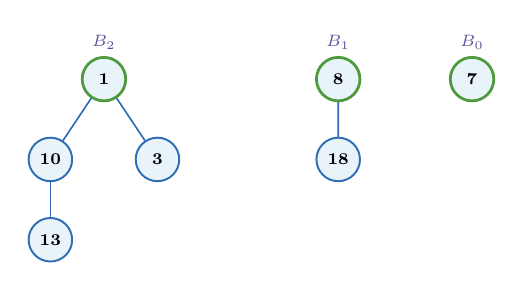
\begin{tikzpicture}[
  nd/.style={circle, draw=heapblue, line width=0.7pt, minimum size=6.5mm, inner sep=0pt, fill=skyfill, font=\scriptsize\bfseries},
  scale=0.85, transform shape
]
% B_2 (root 1)
\node[nd, draw=greenO, line width=1pt] (r1) at (0,0) {1};
\node[nd] (n10) at (-0.8,-1.2) {10};
\node[nd] (n3) at (0.8,-1.2) {3};
\node[nd] (n13) at (-0.8,-2.4) {13};
\draw[heapblue, line width=0.6pt] (r1)--(n10);
\draw[heapblue, line width=0.6pt] (r1)--(n3);
\draw[heapblue, line width=0.6pt] (n10)--(n13);
\node[font=\scriptsize\bfseries\color{violetT}] at (0,0.55) {$B_2$};

% B_1 (root 8)
\node[nd, draw=greenO, line width=1pt] (r8) at (3.5,0) {8};
\node[nd] (n18) at (3.5,-1.2) {18};
\draw[heapblue, line width=0.6pt] (r8)--(n18);
\node[font=\scriptsize\bfseries\color{violetT}] at (3.5,0.55) {$B_1$};

% B_0 (root 7)
\node[nd, draw=greenO, line width=1pt] (r7) at (5.5,0) {7};
\node[font=\scriptsize\bfseries\color{violetT}] at (5.5,0.55) {$B_0$};
\end{tikzpicture}
\end{center}

\textcolor{heapblue}{\textbf{Total key comparisons:}} $0+1+0+2+0+1+0 = 4 = n - \alpha(n) = 7 - 3$
\end{examplebox}

\begin{keybox}[Important Facts]
\renewcommand{\arraystretch}{1.4}
\begin{tabular}{l l}
Each edge & corresponds to exactly \textbf{one key comparison} \\
Building from $n$ elements & takes $\textcolor{violetT}{O(n)}$ key comparisons total \\
\end{tabular}
\end{keybox}

% ==================================================================
\section{Memory Representation}

\subsection{Three Pointers Per Node}

\begin{keybox}[Pointer Structure]
Each node stores \textbf{three pointers} plus two data fields:

\begin{center}
\renewcommand{\arraystretch}{1.4}
\begin{tabular}{l l l}
\hline
\textbf{Field} & \textbf{Points To} & \textbf{Color}\\
\hline
\textcolor{rustW}{\textbf{PARENT}} & Parent node & \textcolor{rustW}{Red}\\
\texttt{key} & Element's key & (data)\\
\texttt{degree} & Number of children & (data)\\
\textcolor{greenO}{\textbf{CHILD}} & Leftmost child & \textcolor{greenO}{Green}\\
\textcolor{heapblue}{\textbf{SIBLING}} & Right sibling & \textcolor{heapblue}{Blue}\\
\hline
\end{tabular}
\end{center}

We need the \textcolor{rustW}{PARENT} pointer for Decrease Key (covered later).
\end{keybox}

\subsection{Visual vs.\ Memory Representation}

\begin{warnbox}[Visual diagram $\ne$ memory pointers]
When we draw a binomial heap, the lines are \textbf{edges} (parent to child).

In memory, the actual \textbf{pointers} are:
\begin{itemize}[leftmargin=1.4em,itemsep=2pt]
  \item \textcolor{rustW}{\textbf{PARENT}}: child $\to$ its parent (upward)
  \item \textcolor{greenO}{\textbf{LEFT CHILD}}: parent $\to$ its \textbf{leftmost} child only
  \item \textcolor{heapblue}{\textbf{RIGHT SIBLING}}: one child $\to$ the next sibling (across)
\end{itemize}
The visual edges are NOT pointers. Each visual edge is implemented through a combination of LEFT CHILD and RIGHT SIBLING pointers.
\end{warnbox}

\subsection{HEAD Pointer and Root List}

The roots of the $B_k$ trees are connected via \textcolor{heapblue}{\textbf{RIGHT SIBLING}} pointers, forming a \textbf{linked list of roots}. A \textbf{HEAD} pointer points to the root of the \textbf{smallest} tree (smallest $k$).

\begin{examplebox}[Memory Layout Example]
Heap: $\langle B_3(\text{root } 8),\; B_2(\text{root } 1),\; B_0(\text{root } 7) \rangle$

Root linked list:

\begin{center}
\texttt{HEAD} $\;\to\;$ \fbox{7} $\;\xrightarrow{\textcolor{heapblue}{\text{sib}}}\;$ \fbox{1} $\;\xrightarrow{\textcolor{heapblue}{\text{sib}}}\;$ \fbox{8} $\;\to\;$ \texttt{NIL}
\end{center}

HEAD points to 7 ($B_0$, smallest tree). Then 7's sibling pointer goes to 1 ($B_2$), then to 8 ($B_3$).

Here is a full pointer diagram for a smaller heap $\langle B_2(\text{root } 3),\; B_1(\text{root } 5),\; B_0(\text{root } 9) \rangle$:

\begin{center}
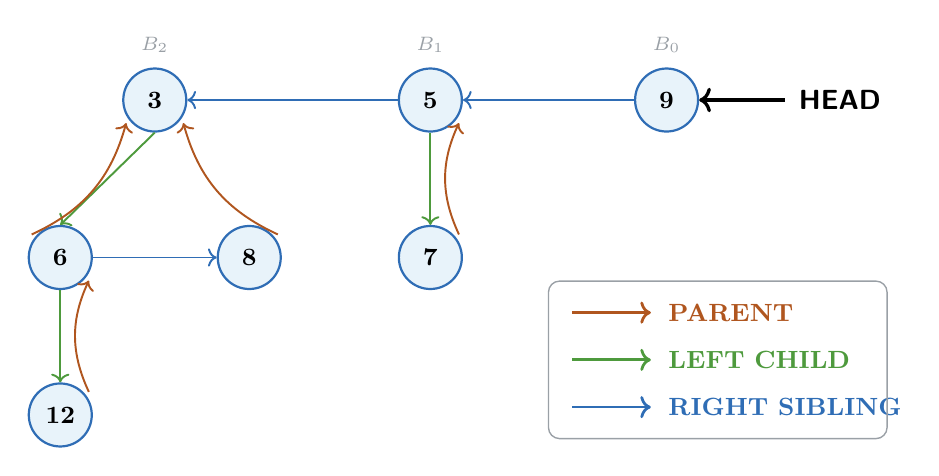
\begin{tikzpicture}[
  nd/.style={circle, draw=heapblue, line width=0.8pt, minimum size=8mm, inner sep=0pt, fill=skyfill, font=\small\bfseries},
]
% Root list (top row)
\node[nd] (n9) at (8,0) {9};
\node[nd] (n5) at (5,0) {5};
\node[nd] (n3) at (1.5,0) {3};

% HEAD
\node[font=\bfseries] at (10.2,0) {\textsf{HEAD}};
\draw[->, line width=1.2pt] (9.5,0) -- (n9);

% Root sibling pointers (blue, right to left)
\draw[->, heapblue, line width=0.7pt] (n9.west) -- (n5.east);
\draw[->, heapblue, line width=0.7pt] (n5.west) -- (n3.east);

% Tree labels above
\node[font=\scriptsize\color{greyline}] at (8,0.7) {$B_0$};
\node[font=\scriptsize\color{greyline}] at (5,0.7) {$B_1$};
\node[font=\scriptsize\color{greyline}] at (1.5,0.7) {$B_2$};

% Under 5 (B_1): left child = 7
\node[nd] (n7) at (5,-2) {7};
\draw[->, greenO, line width=0.7pt] (n5.south) -- (n7.north);
\draw[->, rustW, line width=0.7pt] ([xshift=2pt]n7.north east) to[bend left=25] ([xshift=2pt]n5.south east);

% Under 3 (B_2): left child = 6, sibling = 8
\node[nd] (n6) at (0.3,-2) {6};
\node[nd] (n8) at (2.7,-2) {8};
\draw[->, greenO, line width=0.7pt] (n3.south) -- (n6.north);
\draw[->, heapblue, line width=0.7pt] (n6.east) -- (n8.west);
\draw[->, rustW, line width=0.7pt] ([xshift=-2pt]n6.north west) to[bend right=25] ([xshift=-2pt]n3.south west);
\draw[->, rustW, line width=0.7pt] ([xshift=2pt]n8.north east) to[bend left=25] ([xshift=2pt]n3.south east);

% Under 6: left child = 12
\node[nd] (n12) at (0.3,-4) {12};
\draw[->, greenO, line width=0.7pt] (n6.south) -- (n12.north);
\draw[->, rustW, line width=0.7pt] ([xshift=2pt]n12.north east) to[bend left=25] ([xshift=2pt]n6.south east);

% Legend
\draw[->, rustW, line width=1pt] (6.8,-2.7) -- (7.8,-2.7);
\node[font=\small\bfseries, anchor=west, text=rustW] at (7.9,-2.7) {PARENT};
\draw[->, greenO, line width=1pt] (6.8,-3.3) -- (7.8,-3.3);
\node[font=\small\bfseries, anchor=west, text=greenO] at (7.9,-3.3) {LEFT CHILD};
\draw[->, heapblue, line width=1pt] (6.8,-3.9) -- (7.8,-3.9);
\node[font=\small\bfseries, anchor=west, text=heapblue] at (7.9,-3.9) {RIGHT SIBLING};
\draw[rounded corners, greyline, line width=0.5pt] (6.5,-2.3) rectangle (10.8,-4.3);
\end{tikzpicture}
\end{center}
\end{examplebox}

% ==================================================================
\section{Two Key Lemmas}

Before the operations, we need two building blocks. These lemmas are \textbf{the reason} all operations work efficiently.

\subsection{Lemma 1: Merging Two $B_k$ Trees}

\begin{keybox}[Lemma 1]
We can merge \textcolor{rustW}{two} min heap ordered $B_k$ trees into a \textcolor{greenO}{single} min heap ordered $B_{k+1}$ tree using just \textcolor{violetT}{\textbf{one}} key comparison.
\end{keybox}

\begin{keybox}[Why Lemma 1 Matters]
This is the \textbf{carry operation}. Just like adding two 1 bits produces a carry in binary addition, merging two $B_k$'s produces one $B_{k+1}$. This is the core mechanism behind Union, Insert, and Extract\_Min.
\end{keybox}

\textbf{Proof.} Given two $B_k$ trees with roots $x$ and $y$:

\begin{enumerate}[leftmargin=1.4em,itemsep=3pt]
  \item Compare $x.\text{key}$ and $y.\text{key}$ \quad (one comparison).
  \item Smaller root stays on top. Make the other tree the new leftmost subtree.
\end{enumerate}

If $x \le y$: $x$ is root of $B_{k+1}$, with children $B_k(y),\, B_{k-1},\, \ldots,\, B_0$.

Min heap ordering preserved (smaller root on top). Structure is $B_{k+1}$ by definition. \hfill $\square$

\begin{examplebox}[Lemma 1 in Action: Merging Two $B_1$'s into $B_2$]
Two min heap ordered $B_1$ trees. One comparison decides the root.

\begin{center}
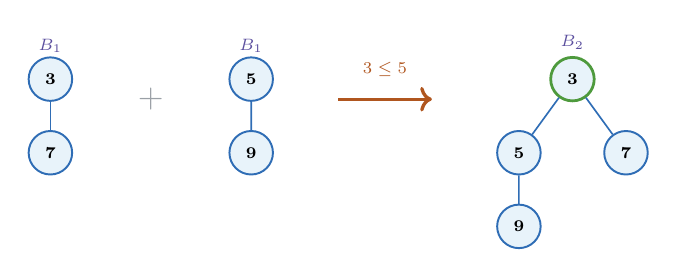
\begin{tikzpicture}[
  nd/.style={circle, draw=heapblue, line width=0.7pt, minimum size=6.5mm, inner sep=0pt, fill=skyfill, font=\scriptsize\bfseries},
  scale=0.85, transform shape
]
% Left B_1
\node[nd] (a) at (0,0) {3};
\node[nd] (a1) at (0,-1.1) {7};
\draw[heapblue, line width=0.6pt] (a)--(a1);
\node[font=\scriptsize\bfseries\color{violetT}] at (0,0.5) {$B_1$};

% Plus
\node[font=\Large\bfseries\color{greyline}] at (1.5,-0.3) {$+$};

% Right B_1
\node[nd] (b) at (3,0) {5};
\node[nd] (b1) at (3,-1.1) {9};
\draw[heapblue, line width=0.6pt] (b)--(b1);
\node[font=\scriptsize\bfseries\color{violetT}] at (3,0.5) {$B_1$};

% Arrow
\draw[->, line width=1.2pt, rustW] (4.3,-0.3) -- (5.7,-0.3);
\node[font=\scriptsize\bfseries\color{rustW}] at (5,0.15) {$3 \le 5$};

% Result B_2
\node[nd, draw=greenO, line width=1pt] (r) at (7.8,0) {3};
\node[nd] (r1) at (7,-1.1) {5};
\node[nd] (r2) at (8.6,-1.1) {7};
\node[nd] (r3) at (7,-2.2) {9};
\draw[heapblue, line width=0.6pt] (r)--(r1);
\draw[heapblue, line width=0.6pt] (r)--(r2);
\draw[heapblue, line width=0.6pt] (r1)--(r3);
\node[font=\scriptsize\bfseries\color{violetT}] at (7.8,0.55) {$B_2$};
\end{tikzpicture}
\end{center}

$3 \le 5$, so 3 stays as root. The other tree (root 5) becomes the \textbf{new leftmost child}. One comparison, one new edge.
\end{examplebox}

\subsection{Lemma 2: Deleting the Root of $B_k$}

\begin{keybox}[Lemma 2]
Deleting \textcolor{rustW}{the root} of a min heap ordered $B_k$ gives a valid \textcolor{greenO}{min binomial heap} of $2^k - 1$ elements.
\end{keybox}

\begin{keybox}[Why Lemma 2 Matters]
This is the key insight behind Extract\_Min. When we extract the minimum (a root of some $B_k$ tree), the remaining children form their own binomial heap. We then Union that new heap back with the rest.
\end{keybox}

\textbf{Proof.} Root of $B_k$ has children $B_{k-1}, B_{k-2}, \ldots, B_1, B_0$.

Delete the root $\Rightarrow$ left with these $k$ subtrees. Each is already min heap ordered (removing the root does not affect subtrees). The sequence $\langle B_{k-1}, \ldots, B_1, B_0 \rangle$ is a valid binomial forest (strictly decreasing $k$ values), so it is a binomial heap of size $2^{k-1} + \cdots + 1 = 2^k - 1$. \hfill $\square$

% ==================================================================
\section{Operations}

\begin{keybox}[The Big Picture]
\textbf{Everything reduces to Union.}
\begin{itemize}[leftmargin=1.4em,itemsep=2pt]
  \item Insert = Union with a tiny heap (single $B_0$)
  \item Extract\_Min = remove a root (Lemma 2 gives a new heap) + Union
  \item Union itself = binary addition using Lemma 1 as the carry
\end{itemize}
Lemma 1 ($O(1)$ merge) and Lemma 2 (delete root $\Rightarrow$ valid heap) are the two pillars.
\end{keybox}

\subsection{Union($T$, $Q$): Merging Two Binomial Heaps}

\begin{defbox}[Union($T$, $Q$)]
\textbf{Input:} two min binomial heaps $T$ and $Q$.\\
\textbf{Output:} a single min binomial heap $S$ containing all elements.

\textbf{Algorithm:} Binary addition!

Each column (bit position $i$) can have 0, 1, 2, or 3 copies of $B_i$ (from $T$, from $Q$, plus possibly a carry from position $i-1$). Process right to left:
\begin{itemize}[leftmargin=1.4em,itemsep=2pt]
  \item \textbf{0 trees}: nothing in $S$, no carry
  \item \textbf{1 tree}: put it in $S$, no carry
  \item \textbf{2 trees}: merge via Lemma 1 into $B_{i+1}$, carry it. Nothing in $S$ at position $i$.
  \item \textbf{3 trees}: put one in $S$, merge the other two into a carry
\end{itemize}
\end{defbox}

\begin{examplebox}[Full Worked Example: Union($T$, $Q$)]
$T$ has size $3 = \langle 11 \rangle_2$, so $T = \langle B_1, B_0 \rangle$.\\
$Q$ has size $7 = \langle 111 \rangle_2$, so $Q = \langle B_2, B_1, B_0 \rangle$.

Result: $3 + 7 = 10 = \langle 1010 \rangle_2$, so $S = \langle B_3, B_1 \rangle$.

\textbf{Concrete values:}
\begin{itemize}[leftmargin=1.4em,itemsep=1pt]
  \item $T$: $B_1$(root 2, child 4). $B_0$(root 3).
  \item $Q$: $B_2$(root 5, children: 7$\to$9 and 10). $B_1$(root 1, child 8). $B_0$(root 6).
\end{itemize}

\begin{center}
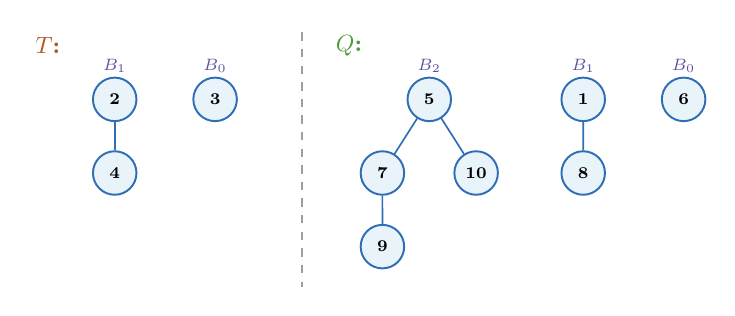
\begin{tikzpicture}[
  nd/.style={circle, draw=heapblue, line width=0.7pt, minimum size=6.5mm, inner sep=0pt, fill=skyfill, font=\scriptsize\bfseries},
  scale=0.85, transform shape
]
% T
\node[font=\bfseries\color{rustW}] at (-0.5,0.8) {$T$:};
\node[nd] (t2) at (0.5,0) {2};
\node[nd] (t4) at (0.5,-1.1) {4};
\draw[heapblue, line width=0.6pt] (t2)--(t4);
\node[font=\scriptsize\color{violetT}] at (0.5,0.5) {$B_1$};
\node[nd] (t3) at (2,0) {3};
\node[font=\scriptsize\color{violetT}] at (2,0.5) {$B_0$};
% divider
\draw[greyline, dashed, line width=0.5pt] (3.3,1) -- (3.3,-2.8);
% Q
\node[font=\bfseries\color{greenO}] at (4,0.8) {$Q$:};
\node[nd] (q5) at (5.2,0) {5};
\node[nd] (q7) at (4.5,-1.1) {7};
\node[nd] (q10) at (5.9,-1.1) {10};
\node[nd] (q9) at (4.5,-2.2) {9};
\draw[heapblue, line width=0.6pt] (q5)--(q7); \draw[heapblue, line width=0.6pt] (q5)--(q10);
\draw[heapblue, line width=0.6pt] (q7)--(q9);
\node[font=\scriptsize\color{violetT}] at (5.2,0.5) {$B_2$};
\node[nd] (q1) at (7.5,0) {1};
\node[nd] (q8) at (7.5,-1.1) {8};
\draw[heapblue, line width=0.6pt] (q1)--(q8);
\node[font=\scriptsize\color{violetT}] at (7.5,0.5) {$B_1$};
\node[nd] (q6) at (9,0) {6};
\node[font=\scriptsize\color{violetT}] at (9,0.5) {$B_0$};
\end{tikzpicture}
\end{center}

\textbf{\textcolor{violetT}{Position 0} ($B_0$ column):}

$T$ has $B_0$(3), $Q$ has $B_0$(6). Two trees $\Rightarrow$ merge.

Compare 3 vs 6: $3 \le 6 \Rightarrow B_1$(root 3, child 6). This is the \textbf{carry}.

$S$ at position 0: empty.\\[6pt]

\textbf{\textcolor{violetT}{Position 1} ($B_1$ column):}

$T$ has $B_1$(root 2), $Q$ has $B_1$(root 1), plus carry $B_1$(root 3). \textcolor{rustW}{Three trees!}

Keep one in $S$: the carry $B_1$(3$\to$6).

Merge the other two: compare 1 vs 2: $1 \le 2 \Rightarrow B_2$(root 1, with subtrees from both). New carry.

$S$ at position 1: $B_1$(root 3, child 6).\\[6pt]

\textbf{\textcolor{violetT}{Position 2} ($B_2$ column):}

$Q$ has $B_2$(root 5), plus carry $B_2$(root 1). Two trees $\Rightarrow$ merge.

Compare 1 vs 5: $1 \le 5 \Rightarrow B_3$(root 1). Carry to position 3.

$S$ at position 2: empty.\\[6pt]

\textbf{\textcolor{violetT}{Position 3} ($B_3$ column):}

Just the carry $B_3$(root 1). One tree $\Rightarrow$ done.

$S$ at position 3: $B_3$(root 1).\\[6pt]

\textbf{\textcolor{violetT}{Result:}} $S = \langle B_3(\text{root } 1),\; B_1(\text{root } 3) \rangle$ \qquad $10 = \langle 1010 \rangle_2$ \checkmark

\begin{center}
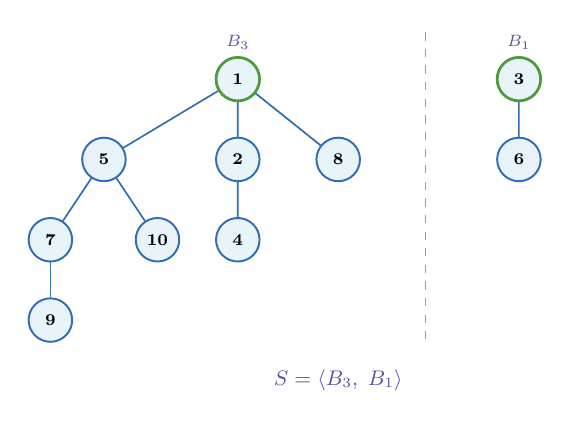
\begin{tikzpicture}[
  nd/.style={circle, draw=heapblue, line width=0.7pt, minimum size=6.5mm, inner sep=0pt, fill=skyfill, font=\scriptsize\bfseries},
  scale=0.85, transform shape
]
% B_3 (root 1)
\node[nd, draw=greenO, line width=1pt] (r1) at (2,0) {1};
\node[font=\scriptsize\bfseries\color{violetT}] at (2,0.55) {$B_3$};
% Children: B_2(5), B_1(2), B_0(8)
\node[nd] (n5) at (0,-1.2) {5};
\node[nd] (n2) at (2,-1.2) {2};
\node[nd] (n8) at (3.5,-1.2) {8};
\draw[heapblue, line width=0.6pt] (r1)--(n5);
\draw[heapblue, line width=0.6pt] (r1)--(n2);
\draw[heapblue, line width=0.6pt] (r1)--(n8);
% Children of 5: B_1(7), B_0(10)
\node[nd] (n7) at (-0.8,-2.4) {7};
\node[nd] (n10) at (0.8,-2.4) {10};
\draw[heapblue, line width=0.6pt] (n5)--(n7);
\draw[heapblue, line width=0.6pt] (n5)--(n10);
% Child of 7: B_0(9)
\node[nd] (n9) at (-0.8,-3.6) {9};
\draw[heapblue, line width=0.6pt] (n7)--(n9);
% Child of 2: B_0(4)
\node[nd] (n4) at (2,-2.4) {4};
\draw[heapblue, line width=0.6pt] (n2)--(n4);

% Separator
\draw[greyline, dashed, line width=0.5pt] (4.8,0.7) -- (4.8,-4);

% B_1 (root 3)
\node[nd, draw=greenO, line width=1pt] (r3) at (6.2,0) {3};
\node[font=\scriptsize\bfseries\color{violetT}] at (6.2,0.55) {$B_1$};
\node[nd] (n6) at (6.2,-1.2) {6};
\draw[heapblue, line width=0.6pt] (r3)--(n6);

% Label
\node[font=\small\bfseries\color{violetT}] at (3.5,-4.5) {$S = \langle B_3,\; B_1 \rangle$};
\end{tikzpicture}
\end{center}

\textbf{\textcolor{heapblue}{New edges:}} 3 \qquad \textbf{\textcolor{heapblue}{Key comparisons:}} 3
\end{examplebox}

\begin{keybox}[Union Complexity]
If $|T| \le n$ and $|Q| \le n$, each heap has $\le \lfloor \log_2 n \rfloor + 1$ trees.

$\Rightarrow$ Union takes $\textcolor{violetT}{O(\log n)}$ comparisons (one per column of the binary addition).
\end{keybox}

\subsection{Insert($T$, $x$): Adding a Single Element}

\begin{defbox}[Insert($T$, $x$)]
\begin{enumerate}[leftmargin=1.4em,itemsep=2pt]
  \item Create a new heap $Q$ containing just $x$ (a single $B_0$).
  \item Return Union($T$, $Q$).
\end{enumerate}
\end{defbox}

\begin{keybox}[Insert = Adding 1 in Binary]
If the last bit is 0 (no $B_0$ exists): place the new $B_0$. Done in $O(1)$.

If the last bit is 1: merge into $B_1$ (carry). If $B_1$ already exists, merge again into $B_2$. This cascading carry can go up to $O(\log n)$ positions, but on average much less.
\end{keybox}

\begin{examplebox}[Insert Example]
Heap $T = \langle B_2, B_0 \rangle$ (5 elements, binary $101$). Insert element $x$.

\begin{enumerate}[leftmargin=1.4em,itemsep=2pt]
  \item $x$ becomes $B_0$. Now two $B_0$'s.
  \item Merge them $\Rightarrow$ one $B_1$ (carry). No $B_1$ exists, so $B_1$ stays.
  \item Result: $\langle B_2, B_1 \rangle$ (6 elements, binary $110$). \checkmark
\end{enumerate}
\end{examplebox}

\subsection{Min($T$): Finding the Minimum}

\begin{defbox}[Min($T$)]
The minimum element is the root of one of the trees (by min heap property).

Walk through the root list (linked list via HEAD pointer). Compare each root's key. Return the smallest.

At most $\lfloor \log_2 n \rfloor + 1$ roots $\Rightarrow$ $\textcolor{violetT}{O(\log n)}$.
\end{defbox}

\subsection{Extract\_Min($T$): Remove the Minimum}

\begin{defbox}[Extract\_Min($T$)]
\begin{enumerate}[leftmargin=1.4em,itemsep=3pt]
  \item \textbf{Find the min:} walk the root list to find the tree $B_k$ whose root has the smallest key. \hfill $O(\log n)$
  \item \textbf{Remove that tree} from the heap $T$. \hfill $O(1)$
  \item \textbf{Delete the root} of $B_k$. By \textbf{Lemma 2}, the children form a new binomial heap $Q = \langle B_{k-1}, \ldots, B_0 \rangle$. \hfill $O(\log n)$
  \item \textbf{Union}$(T, Q)$. \hfill $O(\log n)$
\end{enumerate}
Total: $\textcolor{violetT}{O(\log n)}$.
\end{defbox}

\begin{examplebox}[Extract\_Min Example]
Heap: $\langle B_3(\text{root } 1),\; B_1(\text{root } 3) \rangle$ (10 elements)

\begin{enumerate}[leftmargin=1.4em,itemsep=2pt]
  \item Min = 1 (root of $B_3$).
  \item Remove $B_3$ from heap. Remaining: $\langle B_1(\text{root } 3) \rangle$.
  \item Delete root 1 from $B_3$. Children: $B_2, B_1, B_0$. New heap $Q = \langle B_2, B_1, B_0 \rangle$ (7 elements).
  \item Union($\langle B_1 \rangle$, $\langle B_2, B_1, B_0 \rangle$):

  Position 0: one $B_0$ $\Rightarrow$ stays.

  Position 1: two $B_1$'s $\Rightarrow$ merge into $B_2$ (carry).

  Position 2: two $B_2$'s $\Rightarrow$ merge into $B_3$ (carry).

  Position 3: one $B_3$ $\Rightarrow$ stays.

  Result: $\langle B_3, B_0 \rangle$ (9 elements, $9 = \langle 1001 \rangle_2$) \checkmark
\end{enumerate}

Return 1.
\end{examplebox}

% ==================================================================
\section{Complexity Summary}

\begin{keybox}[Binomial Heap Operations]
\renewcommand{\arraystretch}{1.5}
\begin{tabular}{l c l}
\textbf{\textcolor{violetT}{Operation}} & \textbf{Worst Case} & \textbf{Key Insight}\\
\hline
\texttt{Union($T$, $Q$)} & $\textcolor{violetT}{O(\log n)}$ & binary addition \\
\texttt{Insert($T$, $x$)} & $\textcolor{violetT}{O(\log n)}$ & Union with single $B_0$ \\
\texttt{Min($T$)} & $\textcolor{violetT}{O(\log n)}$ & scan root list \\
\texttt{Extract\_Min($T$)} & $\textcolor{violetT}{O(\log n)}$ & Lemma 2 + Union \\
\end{tabular}
\end{keybox}

% ==================================================================
\section{Practice Problems}

\begin{examplebox}[Problem 1: Build a Binomial Heap]
Build a min binomial heap by inserting: $5, 12, 3, 9, 2, 15, 6, 1$.

(a) How many trees does the final heap have?\\
(b) What is the root of each tree?\\
(c) How many total key comparisons?

\begin{answerband}
$n = 8 = \langle 1000 \rangle_2 \Rightarrow F_8 = \langle B_3 \rangle$ (one tree).

Step by step:
\begin{itemize}[leftmargin=1.4em,itemsep=1pt]
  \item Insert 5: $\langle B_0(5) \rangle$. \hfill 0 comps
  \item Insert 12: merge $B_0$'s: $5 \le 12$. $\langle B_1(5 \to 12) \rangle$. \hfill 1 comp
  \item Insert 3: $\langle B_1(5), B_0(3) \rangle$. \hfill 0 comps
  \item Insert 9: merge $B_0$'s: $3 \le 9$. Two $B_1$'s: $3 \le 5$. $\langle B_2(\text{root } 3) \rangle$. \hfill 2 comps
  \item Insert 2: $\langle B_2(3), B_0(2) \rangle$. \hfill 0 comps
  \item Insert 15: merge $B_0$'s: $2 \le 15$. $\langle B_2(3), B_1(2 \to 15) \rangle$. \hfill 1 comp
  \item Insert 6: $\langle B_2(3), B_1(2), B_0(6) \rangle$. \hfill 0 comps
  \item Insert 1: merge $B_0$'s: $1 \le 6$. Two $B_1$'s: $1 \le 2$. Two $B_2$'s: $1 \le 3$. $\langle B_3(\text{root } 1) \rangle$. \hfill 3 comps
\end{itemize}

(a) \textcolor{violetT}{1 tree.} \quad (b) \textcolor{violetT}{Root is 1.} \quad (c) \textcolor{violetT}{$1+0+2+0+1+0+3 = 7 = n - \alpha(n) = 8 - 1$}
\end{answerband}
\end{examplebox}

\begin{examplebox}[Problem 2: Extract\_Min]
Given: $\langle B_2(\text{root } 3, \text{children: } 7 \to 9 \text{ and } 5),\; B_0(\text{root } 10) \rangle$. Perform Extract\_Min.

\begin{answerband}
\begin{enumerate}[leftmargin=1.4em,itemsep=2pt]
  \item Min = 3 (root of $B_2$). Extract it.
  \item Remove $B_2$. Remaining: $\langle B_0(10) \rangle$.
  \item Root 3 had children: $B_1$(root 7, child 9) and $B_0$(root 5). New heap $Q = \langle B_1(7 \to 9), B_0(5) \rangle$.
  \item Union($\langle B_0(10) \rangle$, $\langle B_1(7), B_0(5) \rangle$):

  Position 0: two $B_0$'s (10, 5). $5 \le 10 \Rightarrow B_1$(root 5, child 10). Carry.

  Position 1: $B_1$(root 7) + carry $B_1$(root 5). $5 \le 7 \Rightarrow B_2$(root 5). Carry.

  Position 2: just carry. Done.

  Result: $\langle B_2(\text{root } 5) \rangle$ (4 elements, $4 = \langle 100 \rangle_2$) \checkmark
\end{enumerate}

Return 3.
\end{answerband}
\end{examplebox}

\begin{examplebox}[Problem 3: Properties Quick Check]
For $B_5$:

\begin{center}
\renewcommand{\arraystretch}{1.3}
\begin{tabular}{l l}
Nodes? & \textcolor{violetT}{$2^5 = 32$} \\
Height? & \textcolor{violetT}{$5$} \\
Degree of root? & \textcolor{violetT}{$5$} \\
Nodes at depth 2? & \textcolor{violetT}{$\binom{5}{2} = 10$} \\
Nodes at depth 5? & \textcolor{violetT}{$\binom{5}{5} = 1$} \\
\end{tabular}
\end{center}

For $F_{13}$ ($13 = \langle 1101 \rangle_2$):

\begin{center}
\renewcommand{\arraystretch}{1.3}
\begin{tabular}{l l}
Which trees? & \textcolor{violetT}{$\langle B_3, B_2, B_0 \rangle$} \\
How many trees? & \textcolor{violetT}{$\alpha(13) = 3$} \\
How many edges? & \textcolor{violetT}{$13 - 3 = 10$} \\
\end{tabular}
\end{center}
\end{examplebox}

% ==================================================================
\section{Exam Relevance}

Based on past CSC263 exams (2012 through 2015), no specific binomial heap questions appeared. However, heap questions show up frequently. The $k$Set ADT problem from Fall 2014 (see Lecture 2 notes) used max heaps and min heaps together.

\begin{warnbox}[What to watch for on binomial heap questions]
\begin{itemize}[leftmargin=1.4em,itemsep=2pt]
  \item ``Draw the binomial heap after inserting $x_1, x_2, \ldots$'' $\Rightarrow$ binary addition method
  \item ``Show the result of Extract\_Min'' $\Rightarrow$ Lemma 2 + Union
  \item ``How many key comparisons?'' $\Rightarrow$ count new edges = count merges
  \item ``Why $O(\log n)$?'' $\Rightarrow$ at most $\lfloor \log_2 n \rfloor + 1$ trees, binary addition has that many columns
\end{itemize}
\end{warnbox}

% ==================================================================
\section*{\textcolor{violetT}{Quick Reference: Lecture 3}}
\addcontentsline{toc}{section}{Quick Reference: Lecture 3}
\begin{keybox}
\renewcommand{\arraystretch}{1.4}
\begin{tabular}{l l}
$B_k$ & two $B_{k-1}$'s merged; has $2^k$ nodes, height $k$, $\binom{k}{d}$ at depth $d$\\
$F_n$ & forest of $B_k$'s matching 1 bits of $n$; has $\alpha(n)$ trees, $n{-}\alpha(n)$ edges\\
Min Binomial Heap & $F_n$ + one element per node + min heap ordering\\
Memory & 3 pointers: \textcolor{rustW}{PARENT}, \textcolor{greenO}{LEFT CHILD}, \textcolor{heapblue}{RIGHT SIBLING}; HEAD $\to$ root list\\
Lemma 1 & merge two $B_k \to B_{k+1}$ with 1 comparison (the ``carry'')\\
Lemma 2 & delete root of $B_k \to$ valid heap of $2^k{-}1$ elements\\
\textbf{Union} & binary addition $\to$ $O(\log n)$\\
\textbf{Insert} & Union with $B_0$ $\to$ $O(\log n)$\\
\textbf{Min} & scan root list $\to$ $O(\log n)$\\
\textbf{Extract\_Min} & Lemma 2 + Union $\to$ $O(\log n)$\\
\end{tabular}
\end{keybox}



\end{document}
